%! Author = alison o'connor
%! Date = 19/10/22
%! Results from PAPERA/BO/RESULTS/V1
%%
%% Copyright 2007-2019 Elsevier Ltd
%%
%% This file is part of the 'Elsarticle Bundle'.
%% ---------------------------------------------
%%
%% It may be distributed under the conditions of the LaTeX Project Public
%% License, either version 1.2 of this license or (at your option) any
%% later version. The latest version of this license is in
%%	http://www.latex-project.org/lppl.txt
%% and version 1.2 or later is part of all distributions of LaTeX
%% version 1999/12/01 or later.
%%
%% The list of all files belonging to the 'Elsarticle Bundle' is
%% given in the file `manifest.txt'.
%%
%% Template article for Elsevier's document class `elsarticle'
%% with harvard style bibliographic references

\documentclass[preprint, review, 12pt]{elsarticle}

%% Use the option review to obtain double line spacing
%% \documentclass[preprint,review,12pt]{elsarticle}

%% The amssymb package provides various useful mathematical symbols
\usepackage{amssymb}
%% The amsthm package provides extended theorem environments
%% \usepackage{amsthm}

%% The lineno packages adds line numbers. Start line numbering with
%% \begin{linenumbers}, end it with \end{linenumbers}. Or switch it on
%% for the whole article with \linenumbers.
%\usepackage{lineno}
%\linenumbers


%% MY PACKAGES
\usepackage{afterpage}
\usepackage{amsmath}
\usepackage{amsfonts}
\usepackage{amssymb}
\usepackage{array}
\usepackage{adjustbox}
\usepackage[bookmarks=false, breaklinks]{hyperref}
\hypersetup{colorlinks,
	linkcolor=blue,
	citecolor=blue,
	urlcolor=blue}
\usepackage{bm}
\usepackage{booktabs}
\usepackage{caption}
\usepackage{float}
\usepackage{gensymb}
\usepackage{wasysym}
\usepackage{import}
\usepackage[utf8]{inputenc}
\usepackage{tabularx}
\usepackage{multicol}
\usepackage{multirow}
\usepackage{siunitx}
\usepackage{subcaption}
\usepackage{placeins}
\usepackage{pdflscape}
\usepackage{longtable}
\usepackage[markup=underlined]{changes}
\newcolumntype{P}[1]{>{\centering\arraybackslash}p{#1}}
\usepackage{graphicx}
\graphicspath{{../../RESULTS/}{../FIGURES/}}
\renewcommand{\floatpagefraction}{.8}%
%%COLUMN WIDTHS FOR TABLES
\newcolumntype{b}{X}
\newcolumntype{s}{>{\hsize=.2\hsize}X}
\newcolumntype{m}{>{\hsize=.5\hsize}X}
\usepackage{soul}
%%%FORMATTING
%\widowpenalty10000
%\clubpenalty10000

\journal{European Journal of Mechanics A/Solids}


\begin{document}
	\begin{frontmatter}


		\title{A Machine Learning Approach to Automate Ductile Damage Parameter Selection in Finite Element Simulations}

		\author[1,2]{A.N. O'Connor\corref{cor1}}
		\ead{alison.oconnor@ul.ie}
		\author[1,3]{P.G. Mongan}
		\author[1,2,3]{N.P. O'Dowd}

		\address[1]{School of Engineering, University of Limerick, Ireland}
		\address[2]{Bernal Institute, University of Limerick, Ireland}
		\address[3]{Confirm Smart Manufacturing Research Centre, Ireland}

		\begin{abstract}
			A key limitation of finite element analysis of material behaviour is accurate modelling of material damage.
			Here Bayesian optimisation, a machine learning technique, is shown to successfully identify material model parameters in a commonly used ductile damage model.
			The Bayesian derived material model parameters result in simulated output with less than 2\% error compared to experimental data.
			The framework detailed here is fully autonomous, requiring data that can be derived from a simple tensile test.
			This framework has been successfully deployed to three datasets of P91 material tested at ambient ($20~\degree$C) and higher ($500~\degree$C) temperatures.
		\end{abstract}

		\begin{highlights}
			\item Material parameters obtained used Bayesian optimisation provide excellent agreement between simulated and experimental data.
			\item Ductile damage parameters are successfully derived for ambient and higher test temperatures.
			\item Required user-defined input such as test data can be easily obtained from standard engineering tests.
		\end{highlights}

		\begin{keyword}
			machine learning;
			Bayesian optimisation;
			ductile damage;
			parameter selection;
		\end{keyword}

	\end{frontmatter}

	%%%%%%%%%%%%%%%%%%%%%%%%%%%
	\section{Introduction}
	\label{h:introduction}

	The tensile test is a standard test method~\cite{ENISO6892} that provides information about the mechanical properties of metallic materials.
	In cases where experimental data are limited finite element (FE) simulations can be used to simulate the mechanical behaviour of materials and examine hypotheses that cannot be experimentally investigated.
	The FE method offers a level of detail not obtainable from analytical solutions but is relatively computationally expensive and ultimately relies on experimental data for validation.
	Ductile damage modelling can be used in conjunction with FE simulations to represent mechanical behaviour of metals under high strain conditions when damage mechanisms are important~\cite{ABBASSI2013, CHAHBOUB2019, ZHANG2021}.
	Such models are generally complex and require calibration parameters that are difficult to derive experimentally or analytically.
	Calibrating a ductile damage modelling can be considered a form of black box optimisation, where the inputs (calibration parameters) and outputs (data in a tensile test) are known but the functional relationship between the calibration parameters and the material mechanical response is unknown.
	Such an optimisation problem can be solved using machine learning, a term used to describe algorithms and/or statistical models that allow computers to select the best method of progression in a problem, without human interaction or explicit programming~\cite{BIKMKHAMETOV2020}.
	In particular, Bayesian optimisation (BO) has been shown to outperform other machine learning algorithms in solving black box optimisation problems~\cite{SNOEK2012}.
	Machine learning algorithms, informed directly by experimental and/or simulation data, have been successfully employed to solve numerous engineering problems across a wide range of applications~\cite{MONGAN2022, LIU2020, HEGDE2020}.
	BO is commonly used in machine learning for artificial neural network (ANN) hyperparameter selection~\cite{DEWANCKER2016, MONGAN2022, BIKMKHAMETOV2020, GHAVAMIAN2021} and has recently been used to identify material parameters in a viscoplastic material model, \citet{RYAN2022}.
	The versatility of BO makes it an attractive method for solving a wide variety of engineering challenges such as: material design ~\cite{ZHANG2020, CHUAQUI2021}, cardiac mechanics~\cite{BOROWSKA2022}, light emission for thin films~\cite{WANKERL2022} and manufacturing process improvements~\cite{MONGAN2022, GUNN2022}.
	In~\cite{ABENDROTH2006, ABBASSI2013, CHAHBOUB2019, CHEN2021} ANNs have been used to assess damage model parameters.
	However, ANNs require a significant number of FE simulations to `train' the model to recognise correlations and relationships between input values and results which is computationally expensive.
	This work demonstrates how BO can be used to automatically identify the material damage model parameters that best match experimental data from a tensile test, reducing the time associated with deriving parameter values and requiring minimal user intervention.
	A similar approach to that used in \citet{RYAN2022} has been adopted, but in this case the approach is applied to ductile damage, using a Gurson model, rather than the rate sensitive viscoplasticity constitutive models examined in \citet{RYAN2022}.

	\section{Material behaviour in FE simulations}
	\label{h:general_material_behaviour}

	A tensile test consists of a standardised specimen geometry that is loaded in one direction until complete separation of the specimen.
	Data are typically expressed in terms of engineering stress and strain ($\sigma_{eng}$ and $\epsilon_{eng}$, respectively), where stress and strain are derived from test measurements of test machine load and specimen displacement, respectively.
	For metals the relationship between stress and strain typically comprises three regions (see Figure~\ref{fig:eng_ss}): a linear region, a strain hardening region where stress increases non-linearly with strain, and a material damage region where stress decreases non-linearly with increasing strain.
	Several key mechanical properties derived from a tensile test are illustrated in Figure~\ref{fig:eng_ss}.
	The yield strength ($\sigma_y$) defines the stress at which material behaviour becomes non-linear.
	The linear region comprises data preceding the yield point of the material and the material stiffness or Young's modulus ($E$) is the slope of the stress-strain curve, as shown in Figure~\ref{fig:eng_ss}.
	Beyond $\sigma_y$ the slope of the stress-strain decreases and a local geometrical discontinuity known as a `neck' forms in the tensile specimen.
	The ultimate tensile strength, $\sigma_{UTS}$, denotes the maximum stress reached in the tensile test; beyond which the specimen's load bearing capacity degrades.
	The strain hardening region occurs for $\sigma_y \leq \sigma \leq \sigma_{UTS}$, as illustrated in Figure~\ref{fig:eng_ss}, and depicts a non-linear stress-strain relationship.
	\begin{figure}[!htbp]
		\centering
		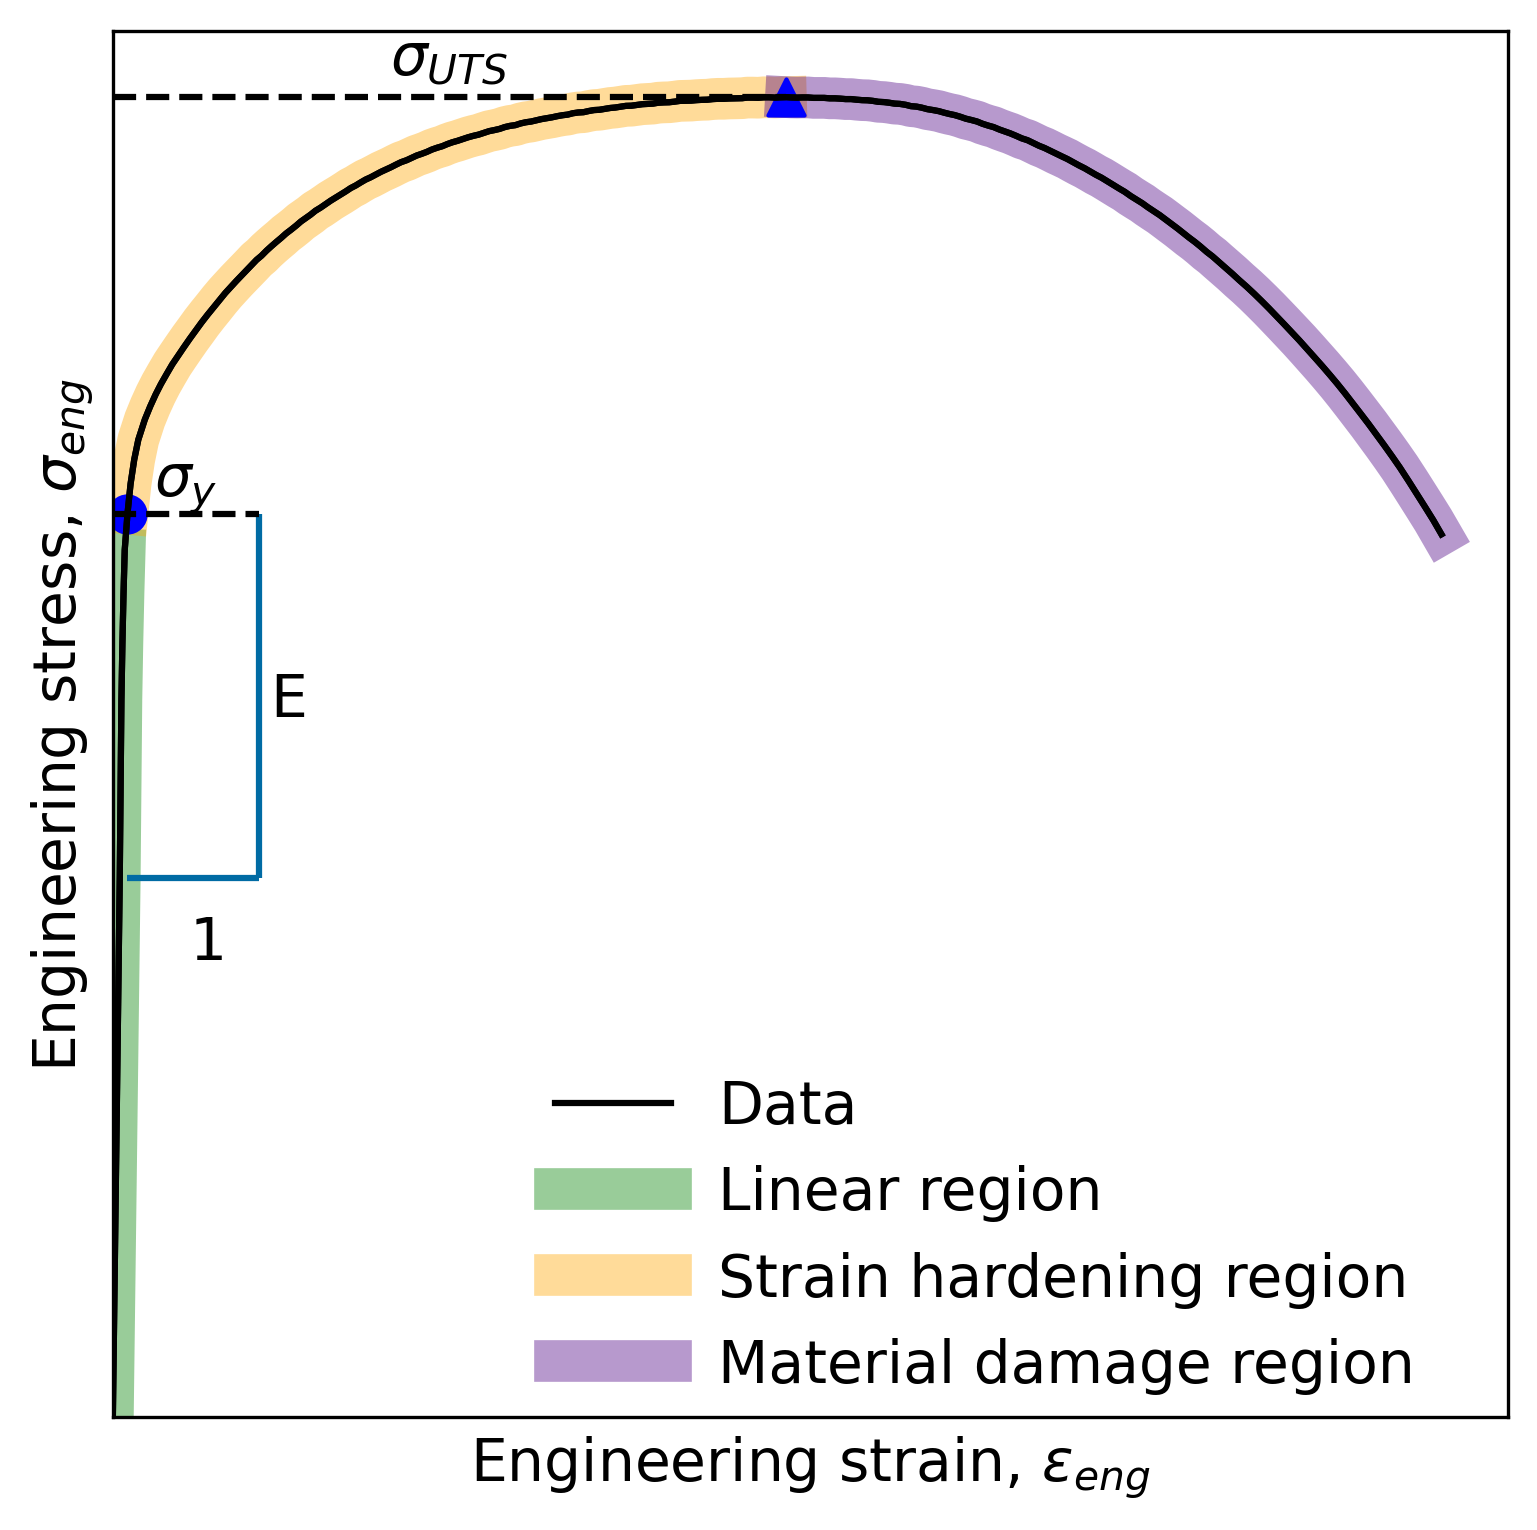
\includegraphics[width=\linewidth, height=0.4\textheight, keepaspectratio]{DIAGRAM_ENG_SS}
		\caption{Illustration depicting material behaviour during tensile test experiment.}
		\label{fig:eng_ss}
	\end{figure}
	The conversion from a load-displacement curve to an engineering stress-strain curve (Equations~\ref{eq:eng_stress}~and~\ref{eq:eng_strain}) used in Figure~\ref{fig:eng_ss}, assumes that the specimen geometry does not change during the test.
		\begin{equation}
		\sigma_{eng} = \frac{P}{A}
		\label{eq:eng_stress}
	\end{equation}

	\begin{equation}
		\varepsilon_{eng} = \frac{\Delta l}{l_o}
		\label{eq:eng_strain}
	\end{equation}
	Where $P$ represents the force applied to the specimen, $A$ the specimen cross-sectional area, $\Delta l$ the change in length of the specimen and $l_0$ the original length.
	However, as the specimen in stretched in the loading direction, in reduces in thickness in the direction transverse to the load, due to the Poisson effect~\cite{YOUNG2001}.
	Therefore, the cross-section area of the specimen decreases continuously with increasing load.
	To account for this geometric change a so-called true stress-true strain relationship (denoted as $\sigma_{true}$ and $\epsilon_{true}$, respectively) is formulated from engineering stress-strain data, as shown in Equations~\ref{eq:eng_stress}~to~\ref{eq:true_strain}~\cite{YOUNG2001}.

	\begin{equation}
		\sigma_{true} = \sigma_{eng} \left( 1 + \varepsilon_{eng} \right)
		\label{eq:true_stress}
	\end{equation}

	\begin{equation}
		\varepsilon_{true} = ln\left( 1 + \varepsilon_{eng} \right)
		\label{eq:true_strain}
	\end{equation}

	This equation becomes increasingly inaccurate as the neck develops due to the non-uniformity of stress and strain in the neck.
	Therefore, in this work for $\sigma > \sigma_{UTS}$, the true stress is interpolated from the values for $\sigma \leq \sigma_{UTS}$, with the understanding that, in the absence of damage, the true stress always increases with increasing strain.
	Here, a linear relationship between true stress and true strain, with slope $m$, for $\sigma \ge \sigma_{UTS}$ is assumed.
	The parameter $m$ is unknown and is calibrated as part of the BO, as discussed later.

	\subsection{The damage model}
	\label{h:damage_model}

	A popular damage model, used to describe the softening behaviour seen in the material damage region of Figure~\ref{fig:eng_ss}, is the Gurson-Tvergaard-Needleman (GTN) model~\cite{WCISLIK2016, CHAHBOUB2019, TVERGAARD1984a}.
	The parameters are typically estimated by conducting numerical simulations, manually iterating the relevant parameter value, and matching the simulation result to experimental data.

	The GTN model response for a tensile test is described in Equation~\ref{eq:gtn_yield}, where $\sigma$ is the current (uniaxial) stress, $\sigma_y$ is the material yield strength, $f$ is the current void volume fraction (the ratio of the volume of voids to the total material volume) and $q_1$, $q_2$, and $q_3$ are material parameters,
	\begin{equation}
		\left( \frac{\sigma}{\sigma_y} \right)^2 + 2q_{1}f\left( \cosh \frac{q_2 \sigma}{2\sigma_y} \right) - q_3 f^2 = 1.
		\label{eq:gtn_yield}
	\end{equation}

	The rate of change of the void volume fraction, $f$, is described by Equation~\ref{eq:vvf} where $\dot{f}_n$ and $\dot{f}_g$ represent the void nucleation rate and void growth rate, respectively,

	\begin{equation}
		\dot{f} = \dot{f}_n + \dot{f}_g.
		\label{eq:vvf}
	\end{equation}
	The void growth rate, $\dot{f}_g$, is obtained from conservation of mass,
	\begin{equation}
		\dot{f}_g = (1-f)\dot{\varepsilon},
		\label{eq:void_growth}
	\end{equation}
	while the void nucleation rate, $\dot{f}_n$, is given by Equation~\ref{eq:void_nucleation}, where $\varepsilon^p_m$ is the plastic strain of the unvoided (matrix) material, and $f_N$, $S_N$ and $\varepsilon_N$, are material parameters.

	\begin{equation}
		\dot{f}_n = \frac{f_N}{S_N \sqrt{2\pi}} \exp \left[ -\frac{1}{2} \left( \frac{{\varepsilon}_m^p -\varepsilon_N}{S_N} \right) ^ 2 \right] \dot{\varepsilon}_m^p,
		\label{eq:void_nucleation}
	\end{equation}

	Since, the void volume, $f$, is defined through a rate equation, the initial void volume fraction, $f_0$, must also be defined.
	Hence, there are a total of seven parameters in the GTN ductile damage model to fit using BO: $q_1$, $q_2$, $q_3$, $S_N$, $f_N$, $\varepsilon_N$, and $f_0$.
	Including the slope of the true stress-true strain curve for $\sigma>\sigma_{UTS}$, $m$, gives a total of eight parameters.

	\section{The Bayesian Optimisation Framework}
	\label{h:general_bo}

	The goal of BO is to find the global minimum of an unknown (black box) function.
	There are two key ingredients to a BO framework: a surrogate model and a loss function.
	The surrogate model, sometimes called a probabilistic model, describes the BO's current knowledge about the unknown function based on observed data.
	The loss function describes how well the previously observed data are optimised (i.e.\ converging towards a global minimum)~\cite{SHAHRIARI2016}.
	The surrogate model and loss function work jointly with an acquisition function, which controls how the BO explores the parameter space.
	The surrogate model, $f(x)$, is determined using Gaussian process regression (GPR) on inputs, $x$, the observed data related to the unknown function.
	A Gaussian process is a collection of random variables, many of which have consistent, joint Gaussian distributions, specified by the covariance function~\cite{RASMUSSEN2004, RASMUSSEN2006} (see Section~\ref{h:covariance_function} for further details on the covariance function).

	The probability distribution generated by GPR is based on a ranking system, where input $x$ is evaluated as $f(x)$ and $f(x)$ is ranked in terms of its performance relative to the loss function.
	In this work the loss function is the mean average percentage error (MAPE) which quantifies the similarity between simulated and experimental data (see Section~\ref{h:mape_detailed} for further detail).
	To minimise the loss function the L-BFGS-B optimisation algorithm~\cite{ZHU1997} is used.
	This algorithm uses historical gradient evaluations of $f(x)$ to construct an approximation of the unknown function.

	In order to set reasonable bounds to the possible solutions of the problem, a parameter space is defined, within which the BO algorithm searches for values.
	The parameter space of the current problem is defined in Table~\ref{tab:parameter_space_all} for the GTN parameters, based on information in the literature for similar materials~\cite{KIRAN2014,MEADE2020,DASSAULT2021}.
	The process used to define the bounds for $m$ is outlined in detail in Section~\ref{h:tensile_tests}.

	\begin{table}[!htbp]
\centering
\caption{Parameter space representing the minimum and maximum boundary for each parameter}
\label{tab:parameter_space_all}
\begin{tabular}{lccc}
\toprule
\textbf{Dataset} &  \textbf{Parameter} & \textbf{Minimum} & \textbf{Maximum}\\
\midrule
%{1-3} &    \textbf{$q_1$} &  0.90 &    1.60 \\
%{1-3} &    \textbf{$q_2$} &  0.90 &    1.10 \\
%{1-3} &    \textbf{$q_3$} &  0.81 &    2.56 \\
%{1-3} &    \textbf{$\epsilon_N$} &  0.25 &    0.40\\
%{1-3} &    \textbf{$f_N$} &  0.03 &    0.09 \\
%{1-3} &    \textbf{$s_N$} &  0.10 &    0.20 \\
%{1-3} &    \textbf{$f_0$} &  1.3\times 10^{-3} &    1.5\times 10^{-3} \\
%{1} &    \textbf{$m$} &  0 &  800 \\
%{2} &    \textbf{$m$} &  0 &  1100 \\
%{3} &    \textbf{$m$} &  0 &  800 \\
%% 3 SIGNIFICANT FIGURES
{1-3} &    \textbf{$q_1$} &  9.00\times 10^{-1} &    1.60 \\
{1-3} &    \textbf{$q_2$} &  9.00\times 10^{-1} &    1.10 \\
{1-3} &    \textbf{$q_3$} &  8.10\times 10^{-1} &    2.56 \\
{1-3} &    \textbf{$\epsilon_N$} &  2.50\times 10^{-1} &    4.00\times 10^{-1}\\
{1-3} &    \textbf{$f_N$} &  3.00\times 10^{-1} &    9.00\times 10^{-2} \\
{1-3} &    \textbf{$s_N$} &  1.00\times 10^{-1} &    2.00\times 10^{-1} \\
{1-3} &    \textbf{$f_0$} &  1.30\times 10^{-3} &    1.50\times 10^{-3} \\
{1} &    \textbf{$m$} &  0 &  800 \\
{2} &    \textbf{$m$} &  0 &  1100 \\
{3} &    \textbf{$m$} &  0 &  800 \\
\bottomrule
\end{tabular}
\end{table}


 	%%%%%%%%%%%%%%%%%%%%%%%%%%%
	\subsection{The covariance function}
	\label{h:covariance_function}

	The covariance function used in the GPR has significant influence on the shape and characteristics of the surrogate function~\cite{MONGAN2022}.
	In this work a covariance function, $k(x_i, x_j)$, which uses a combination of the Mat\'ern, Constant and White noise (White) functions, as shown in Equation~\ref{eq:mykernel}, is implemented,

	\begin{equation}
		k(x_i, x_j) = \text{Mat\'ern} + \text{Constant} \times \text{White}.
		\label{eq:mykernel}
	\end{equation}
	As the shape and/or characteristics of the black box function are unknown this covariance kernel is designed to account for shifts in mean position (Constant), noise (White) and to model potentially multiple minima positions (Mat\'ern).
	Specifically, the Mat\'ern covariance function is defined in Equation~\ref{eq:matern}~\cite{PEDREGOSA2011},
	\begin{equation}
		k(x_i, x_j) = \frac{1}{\Gamma \left( \nu \right)2^{\nu-1}} \left( \frac{\sqrt{2\nu}}{l} d\left( x_i, x_j \right) \right)^{\nu}K_{\nu} \left( \frac{\sqrt{2\nu}}{l} d\left( x_i, x_j \right) \right).
		\label{eq:matern}
	\end{equation}
	In Equation~\ref{eq:matern} $x_i$ and $x_j$ are input points, $d$ is the Euclidean distance, $K_{\nu}$ is a modified Bessel function and $\Gamma$ is the gamma function.

	 The Constant covariance function, is defined in Equation~\ref{eq:constant_kernal}~\cite{PEDREGOSA2011},
	\begin{equation}
		k\left( x_i, x_j \right) = C; \forall \; x_i, x_j,
		\label{eq:constant_kernal}
	\end{equation}
	where $C$ is a constant.

	The White covariance function is defined in Equation~\ref{eq:white},
	\begin{equation}
		k(x_i, x_j) = \sigma^2 \delta_{ij},
		\label{eq:white}
	\end{equation}
 	where $\sigma^2$ is constant and $\delta_{ij}$ the Kronecker delta function.
	In this work the following hyperparameters are fixed: $\nu=1$, $l=1$, $C=1$, $\sigma^2=1$ with the bounds, for each kernel hyperparameter, restricted to: $(1\times10^{-5}, 1\times10^{5})$.
	\textcolor{blue}{the white function seems very simple and not very different from a constant. I'm not sure how that is supposed to represent noise}
	\textcolor{red}{The white noise function adds noise on the diagonal of the matrix to account for uncertainity in data.}
	\textcolor{red}{If input values for kernel are idenitical $(x_i==x_j)$ then the matrix will have a valid of 1 on the diagonal, else it be 0.}
	\textcolor{red}{For FE simulations this may relate to uncertainities in stresses due to meshing or model assumptions.}
	\textcolor{red}{The constant kernel does not depend on inputs.}
	\textcolor{red}{It's main use is to check for bias in the model.}
	\textcolor{red}{By adding a constant to the kernel matrix the model should become less sensitive to small changes in the input values - the idea behind this is that it will improve the numerical stability of the GPR.}

	\textcolor{blue}{I don't understand - your define hyperparameters and then you define bounds}
	\textcolor{red}{These bounds relevant for hyperparameter tuning and must be defined for coding purposes.
	\textcolor{red}{The bounds are given default values and are not modified par for course.}

	\subsection{The loss function}
	\label{h:mape_detailed}

	The aim of this work is to minimise the difference between experimental test data and simulation outputs generated from a finite element (FE) analysis of the problem.
	The experimental data are measures of applied load and specimen extension taken in-situ.
	In this work mean average percentage error (MAPE), Equation~\ref{eq:mape}, is used to measure the similarity between experimental data and simulated output.
 	\begin{equation}
	\text{MAPE} = \frac{100}{n} \sum_i^n \left| \frac{P_{exp}^i - P_{sim}^i}{P_{exp}^i} \right|.
	\label{eq:mape}
	\end{equation}

	Here $P^i_{exp}$ represents each experimental load data point, $P_{sim}^i$ is the corresponding simulation load and $n$ the number of data points.
	MAPE provides an average measure of error over the full dataset with all data points equally weighted.

	%%%%%%%%%%%%%%%%%%%%%%%%%%%
	\subsection{The acquisition function}
	\label{h:acquisition_function}

	In this work the upper confidence bound (UCB) acquisition function is employed.
	The UCB, Equation~\ref{eq:ucb}, identifies the new parameters through a weighted sum of the surrogate function, where $\mu \left(x \right)$ is the mean, and $\sigma \left(x \right)$, the variance, respectively~\cite{SHAHRIARI2016, DEATH2021}.
	\textcolor{blue}{You've previously used $\sigma$ as variance}
	\textcolor{red}{variance and uncertainty used interchangably. Have confirmed it is variance modified accordingly.}

	\begin{equation}
	\alpha_{UCB} \left( x \right) = \mu \left( x \right) + \Beta \: \sigma\left( x \right).
	\label{eq:ucb}
	\end{equation}

	Exploration and exploitation balance how the model searches the parameter space.
	When $\Beta$ is large the acquisition function operates in exploratory mode; reducing the weight switches the model to exploitation mode.
	\textcolor{blue}{Is the weight B or square root of B?}
	\textcolor{red}{The weight is square root of B but others often replace this with Beta symbol as shown above}
	In exploration mode the new assessment point differs significantly from the previous iteration; exploratory mode returns a new assessment point close to that tested previously.
	In our work we have taken $B=2.5$.

	In addition to the weight, $B$, the acquisition function has two further hyperparameters: the number of random samples, $N_R$, and the number of optimisation samples, $N_O$.
	$N_R$ controls the size of the array over which the range of possible inputs are distributed---increasing $N_R$ increases the precision of the GPR, thus reducing uncertainty.
	$N_O$ defines how many evaluations of the acquisition function are conducted and controls the level of uncertainty in the acquisition function---increasing $N_O$ makes the optimisation process more robust.
	\textcolor{red}{Not sure what `----' means}

	\subsection{Initialising the BO framework}
	\label{h:framework}

	BO requires a database of initial evaluated data within the parameter space.
	We use a design of experiment (DoE) approach,~\cite{UY2009, FRALEY2020}, to provide the initial evaluated data.
	DoE maximises the statistical significance of results with a minimised number of experiments.
	Table~\ref{tab:L12} shows a DoE array for 12 initial finite element simulations based on the maximum and minimum parameter space values, where values of 1 and 2 in Table~\ref{tab:L12} represent the minimum and maximum parameter bounds, respectively.

	\begin{table}[tb]
\centering
\caption{Design of experiments array for 8 parameters with each parameter at 2 levels.}
\label{tab:L12}
\begin{tabular}{lrrrrrrrr}
\toprule
{} & $P_1$ & $P_2$ & $P_3$ & $P_4$ & $P_5$ & $P_6$ & $P_7$ & $P_8$ \\
\midrule
\textbf{1 } &     1 &     1 &     1 &     1 &     1 &     1 &     1 &     1 \\
\textbf{2 } &     1 &     1 &     1 &     1 &     1 &     2 &     2 &     2 \\
\textbf{3 } &     1 &     1 &     2 &     2 &     2 &     1 &     1 &     1 \\
\textbf{4 } &     1 &     2 &     1 &     2 &     2 &     1 &     2 &     2 \\
\textbf{5 } &     1 &     2 &     2 &     1 &     2 &     2 &     1 &     2 \\
\textbf{6 } &     1 &     2 &     2 &     2 &     1 &     2 &     2 &     1 \\
\textbf{7 } &     2 &     1 &     2 &     2 &     1 &     1 &     2 &     2 \\
\textbf{8 } &     2 &     1 &     2 &     1 &     2 &     2 &     2 &     1 \\
\textbf{9 } &     2 &     1 &     1 &     2 &     2 &     2 &     1 &     2 \\
\textbf{10} &     2 &     2 &     2 &     1 &     1 &     1 &     1 &     2 \\
\textbf{11} &     2 &     2 &     1 &     2 &     1 &     2 &     1 &     1 \\
\textbf{12} &     2 &     2 &     1 &     1 &     2 &     1 &     2 &     1 \\
\bottomrule
\end{tabular}
\end{table}


	Figure~\ref{fig:doe_flowchart} shows a flowchart describing the DoE procedure.
	As illustrated in Figure~\ref{fig:doe_flowchart}, the user first defines the parameter space (here shown in Table~\ref{tab:parameter_space_all}).
	A DoE array (Table~\ref{tab:L12}) is defined and the array is then modified so that the minimum and maximum values are replaced by the user-defined parameter values.
	A finite element simulation is conducted for each row of the DoE array ($i_{max}$ is the number of (virtual) experiments in the DoE array, here 12.
	Results from the simulation are processed and the experiment data are compared to the simulation data, and the MAPE is calculated.
	After each analysis, $i$, the parameter values and the associated error measurement are appended to a csv file.
	\textcolor{blue}{note: these are not mathematical iterations but are computing iterations! - check the definition on wikipedia, }
	\textcolor{red}{Iteration: the repetition of a process to generate a sequence of outcomes. I'm not clear on where I'm misusing the word iterate?}
	\textcolor{blue}{remove the box around the text "Proceed..." in the figure.}
	\textcolor{red}{done}
	\begin{figure}[!htbp]
		\centering
		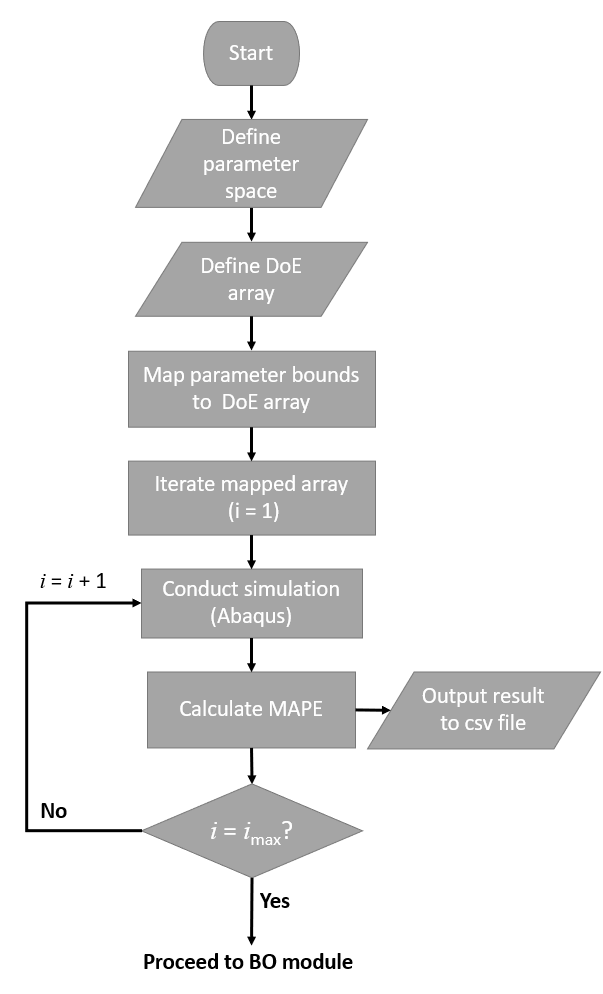
\includegraphics[width=\linewidth, height=0.8\textheight, keepaspectratio]{DOE_FLOWCHART}
		\caption{Flowchart demonstrating the design of experiments code procedure (prior to bayesian optimisation).}
		\label{fig:doe_flowchart}
	\end{figure}

	\subsection{Implementation of the BO-Finite element model}
	\label{h:bayesian_opt}
	The output of the DoE in Figure~\ref{fig:doe_flowchart} (a csv file of parameter values and error measurements) is used to initialise the Bayesian optimiser.
	Figure~\ref{fig:bo_flowchart} outlines the method: The DoE data are analysed by the GPR to create an initial surrogate model.
	GPR outputs are then provided to the acquisition function which identifies new parameter values based on ranking the DoE data.
	A new finite element simulation, using parameter values obtained from the acquisition function, is then conducted.
	Again simulation data is compared to the experiment and the MAPE is calculated.
	Acquisition function parameter values and error measurement data are appended to the existing csv file.
	\textcolor{blue}{please reorganise spacing to avoid double spacing after periods}.
	\textcolor{red}{I will continue to do this}
	The algorithm iterates until the MAPE is less than 2\% or a maximum number of iterations ($j_{max}$) is achieved.
	In the current approach, to ensure that BO is always carried out the analysis is not terminated if MAPE is less than 2\% in the DoE.

	\begin{figure}[!htbp]
		\centering
		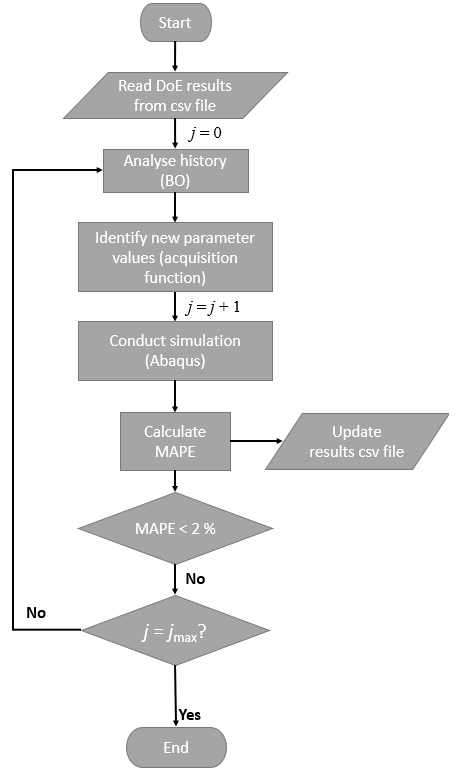
\includegraphics[width=\linewidth, height=0.8\textheight, keepaspectratio]{BO_FLOWCHART}
		\caption{Flowchart depicting code procedure for Bayesian optimisation.}
		\label{fig:bo_flowchart}
	\end{figure}

	%%%%%%%%%%%%%%%%%%%%%%%%%%%
	\section{Experimental Tensile Tests}
	\label{h:tensile_tests}

	The three experimental tensile test results are shown in Figure~\ref{fig:exp_test_results} for the material of interest (P91, a piping steel).
	Datasets 1 \& 2 were conducted under identical test conditions.
	Therefore Dataset 2 can be considered a `repeat' test result.
	\begin{figure}[!htbp]
		\centering
		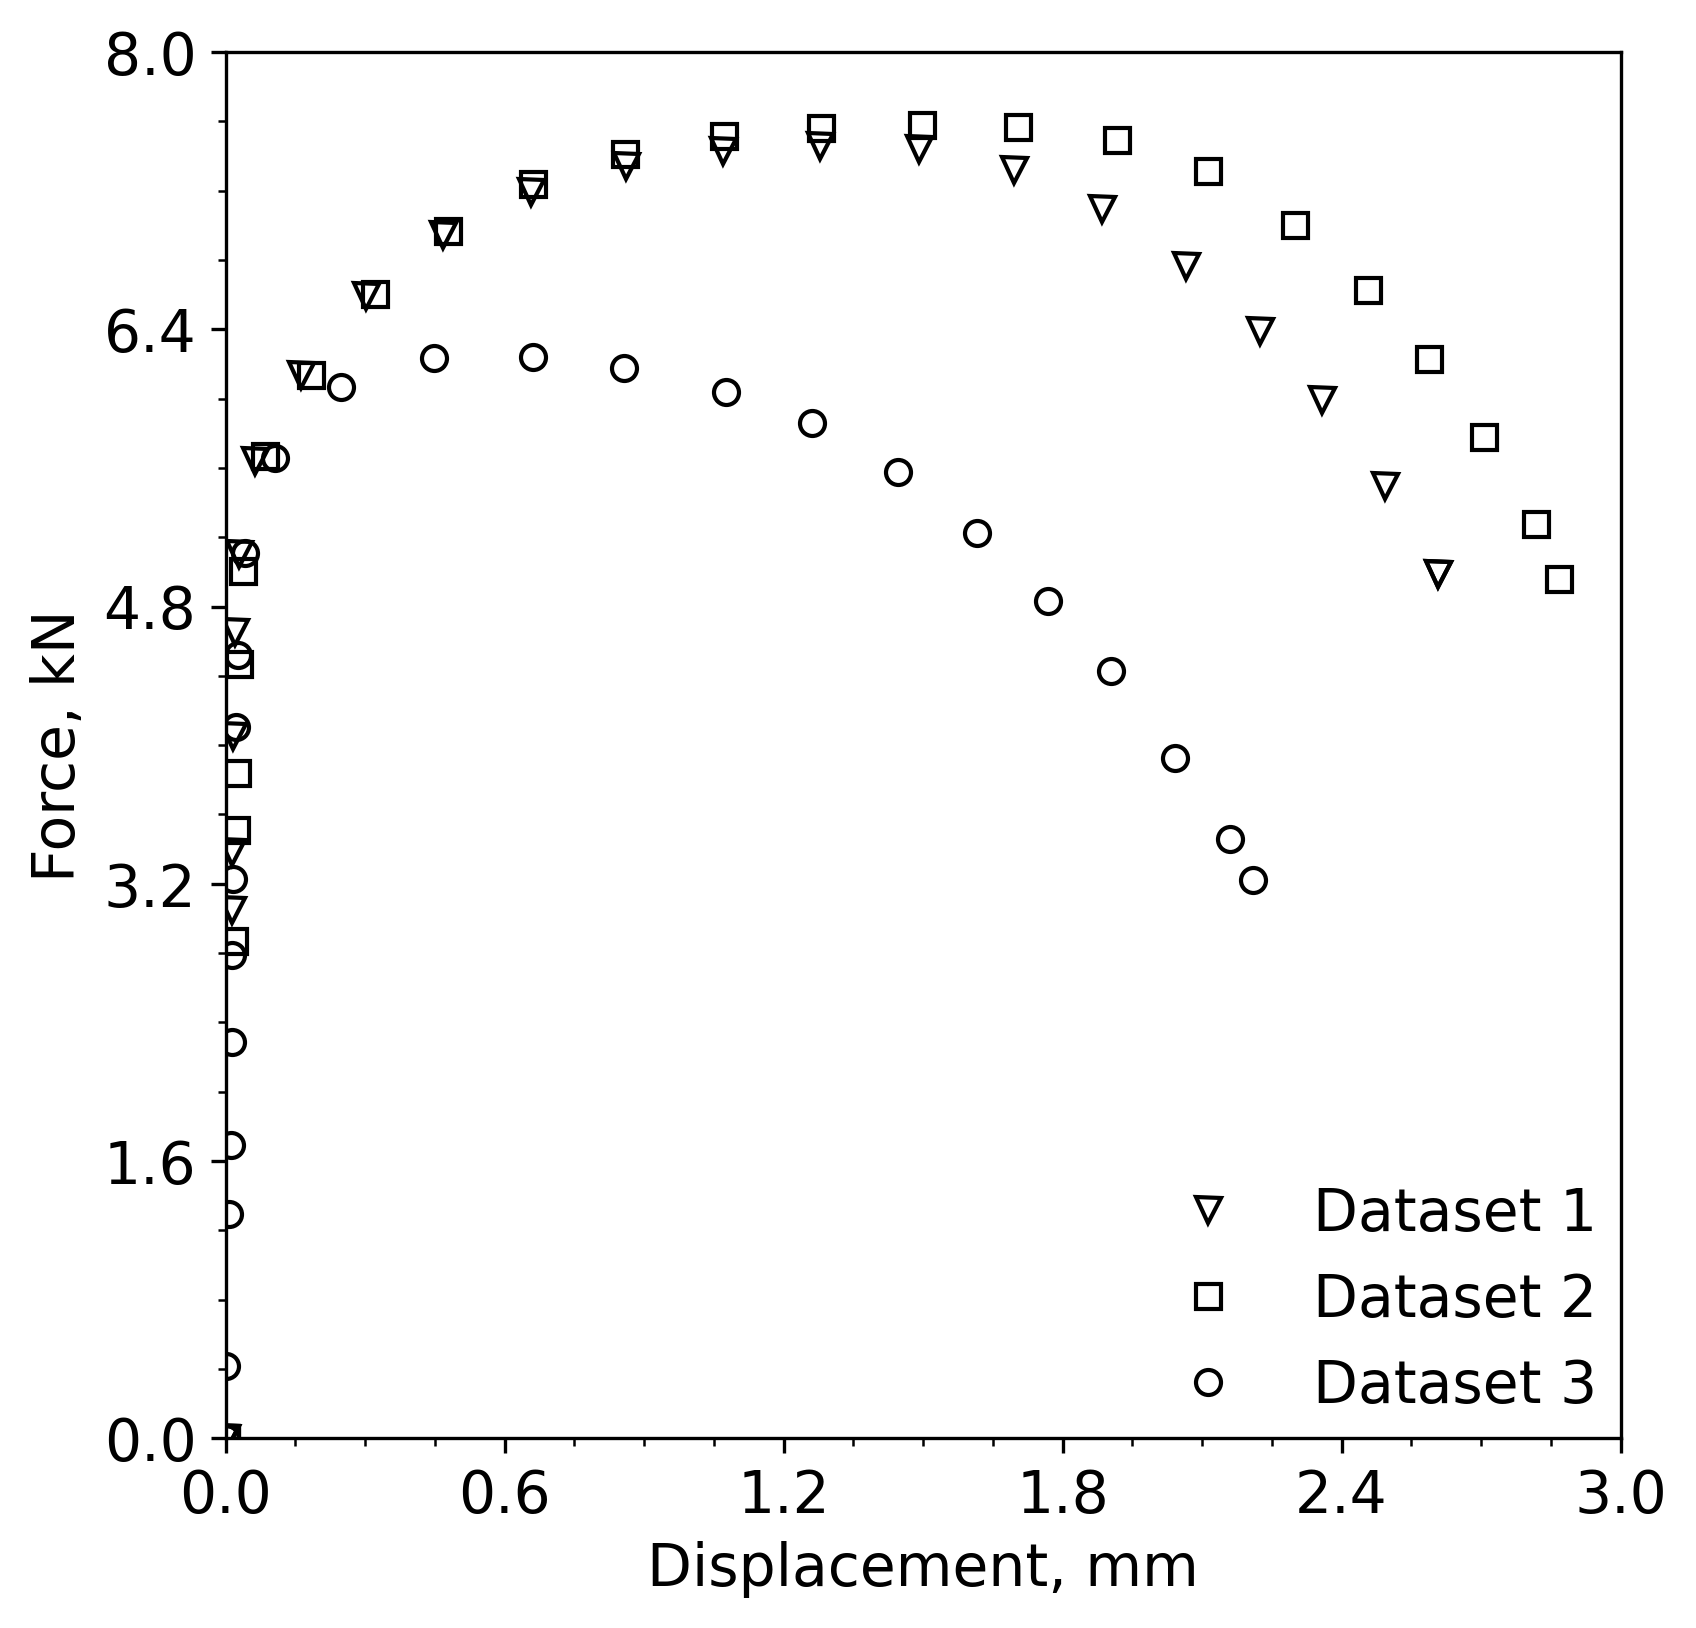
\includegraphics[width=\linewidth, height=0.4\textheight, keepaspectratio]{EXPERIMENTAL_RESULTS}
		\caption{Experimental tensile test results for P91 material at test temperatures of 20~\degree C (Datasets 1 and 2) and 500~\degree C (Dataset 3). Note: Markers are placed as specific intervals for data visibility purposes. Higher data acquistion rate was used during testing.}
		\label{fig:exp_test_results}
	\end{figure}
	Load-displacement data were converted to true stress-strain by limiting data to the range below the maximum load.

	The ultimate tensile strength ($\sigma_{UTS}$) was defined as the true stress corresponding to the maximum load.
	The second derivative of true strain was calculated using a Savitzy-Golay filter with a three degree polynomial fit.

	\subsection{Assessment of linear data}
	\label{h:linear_region}

	To ensure the yield strength was accurately defined the size of the filter window (i.e.\ the number of data points over which the polynomial is applied) was solved iteratively.
	For each iteration (i.e.\ each window size) the yield strength ($\sigma_y$) was defined as the position of the inflection point.
	The `best' yield strength was selected as a function of the error (between the predicted linear region and the experimental linear region), the overall fit of the linear region ($r^2$) and the estimated yield strength value.
	Young's modulus was calculated by employing linear regression to fit all data below the proposed `best' yield strength.
	Figure~\ref{fig:linear_region} shows the result of the assessment for each of the three datasets.

	\begin{figure}[!htbp]
		\centering
		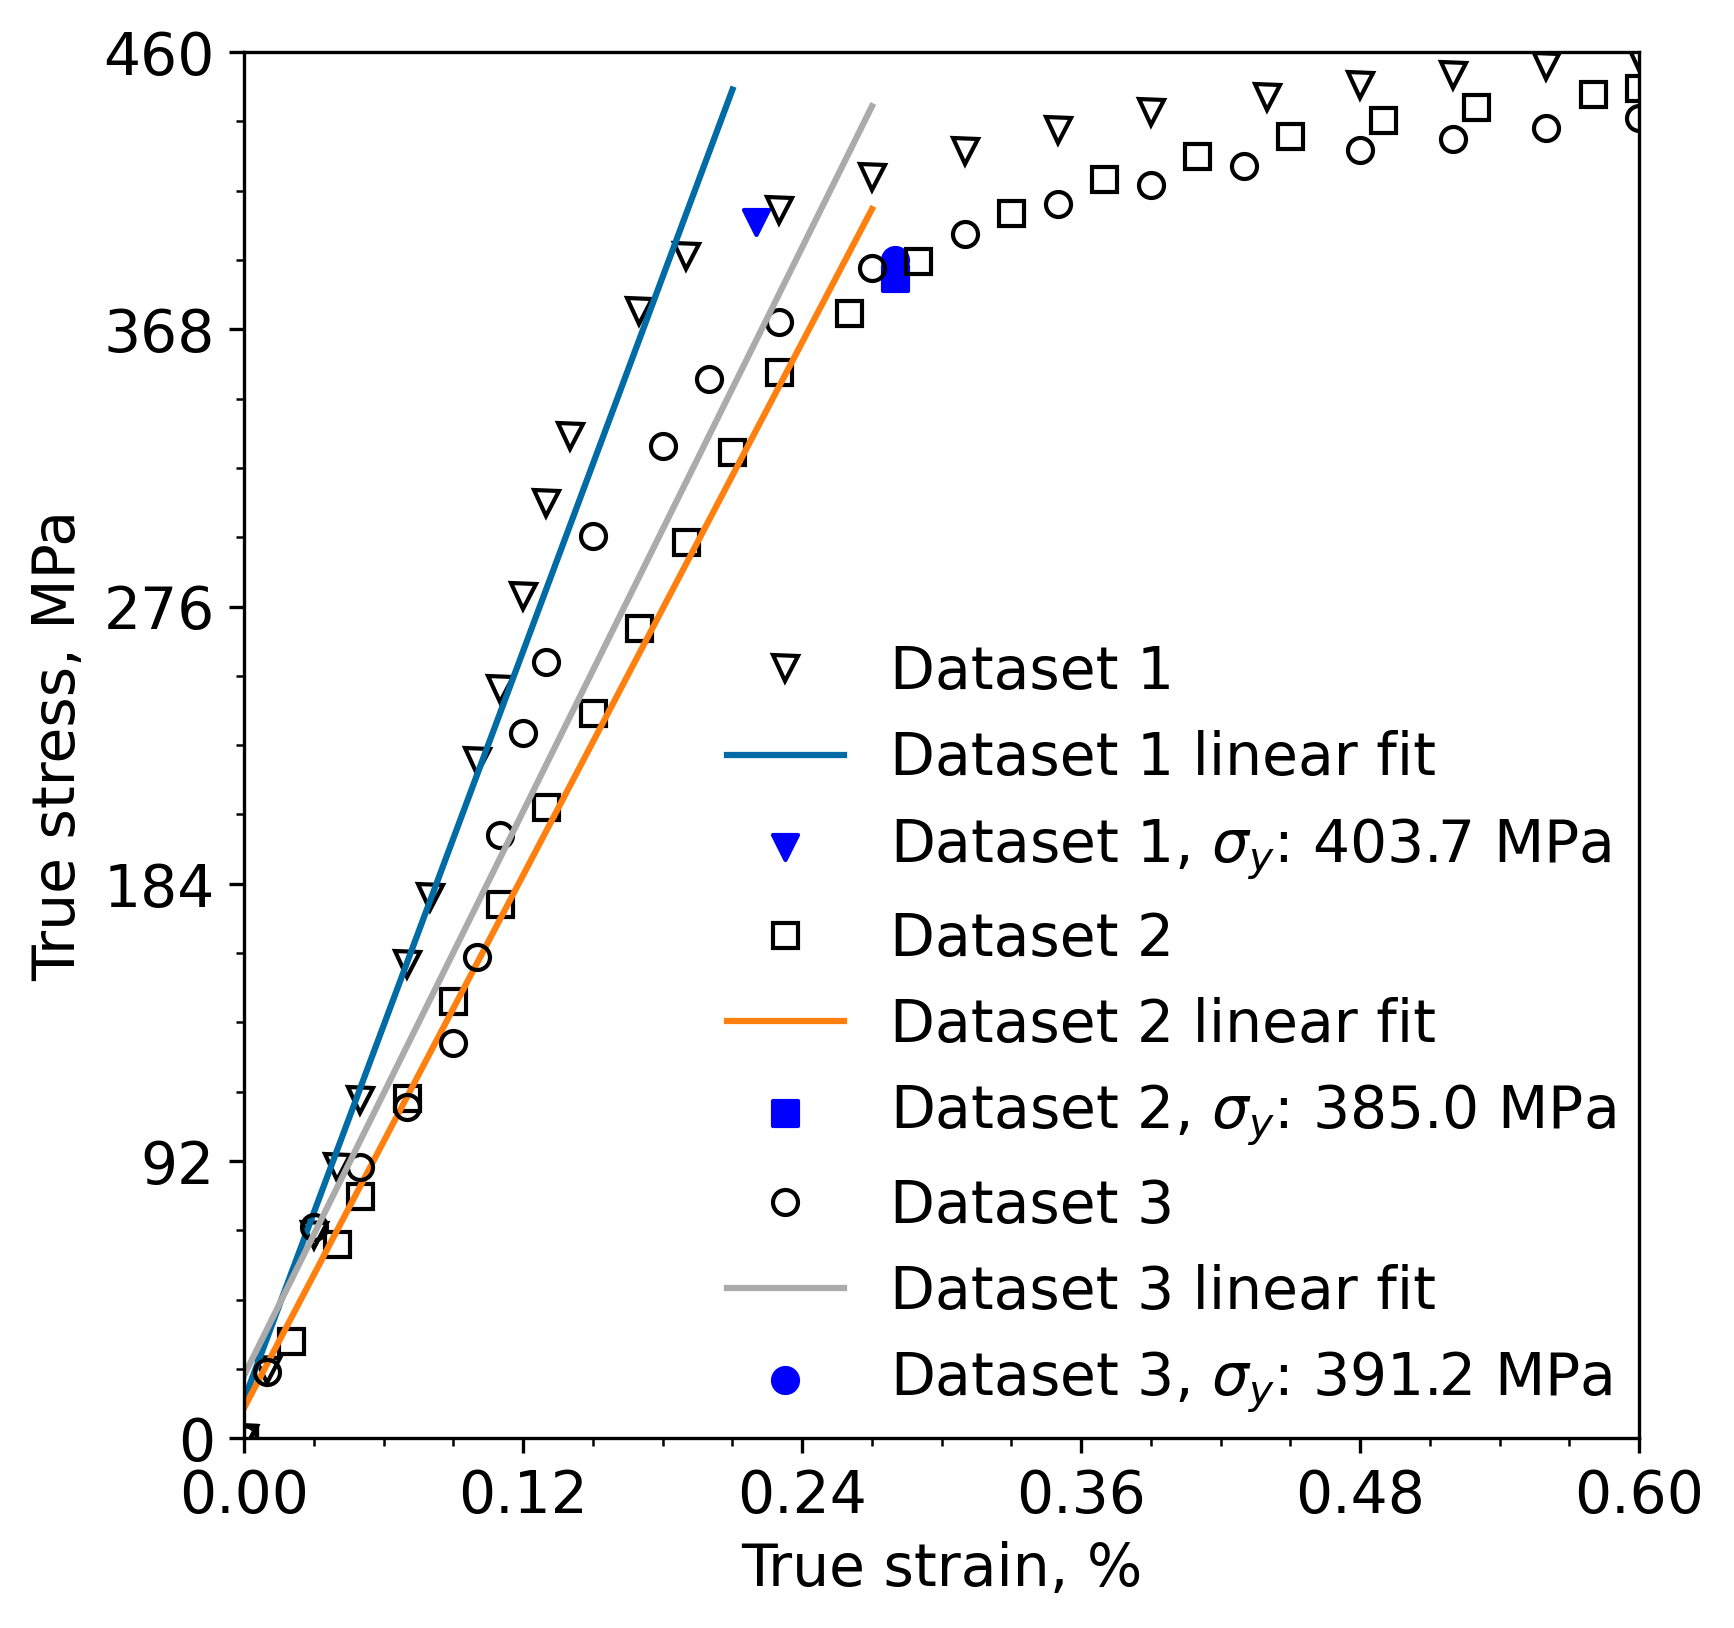
\includegraphics[width=\linewidth, height=0.4\textheight, keepaspectratio]{SECOND_DERIV}
		\caption{True stress - true strain relationship for three experimental tests.}
		\label{fig:linear_region}
	\end{figure}

	To extrapolate data beyond $\sigma_{UTS}$ a linear relationship between stress and strain was assumed.
	The slope of the extrapolated line, parameter $m$, is a searchable parameter that the BO framework will derive.
	The maximum value of parameter $m$ was ascertained from experimental data by applying a linear fit to groups of data preceeding the $\sigma_{UTS}$ position.
	The first fit was applied to a single pair of data points immediately adjacent to the $\sigma_{UTS}$ position, the second fit was applied to the previous pair plus an additional data point, the third fit was applied by expending the second group by an additional data point and so on.
	This method was applied up to a maximum of five data points preceding the $\sigma_{UTS}$ position.
	Parameter $m$ was assessed for each linear fit and the largest value was selected to represent the maximum parameter boundary.
	True stress-true strain data were extrapolated based on the assumption that the extrapolated line must pass through the $\sigma_{UTS}$ position with a slope of parameter $m$.
	Figure~\ref{fig:extending_uts} shows the extrapolated data for the parameter space of dataset 1.
	\begin{figure}[!htbp]
		\centering
		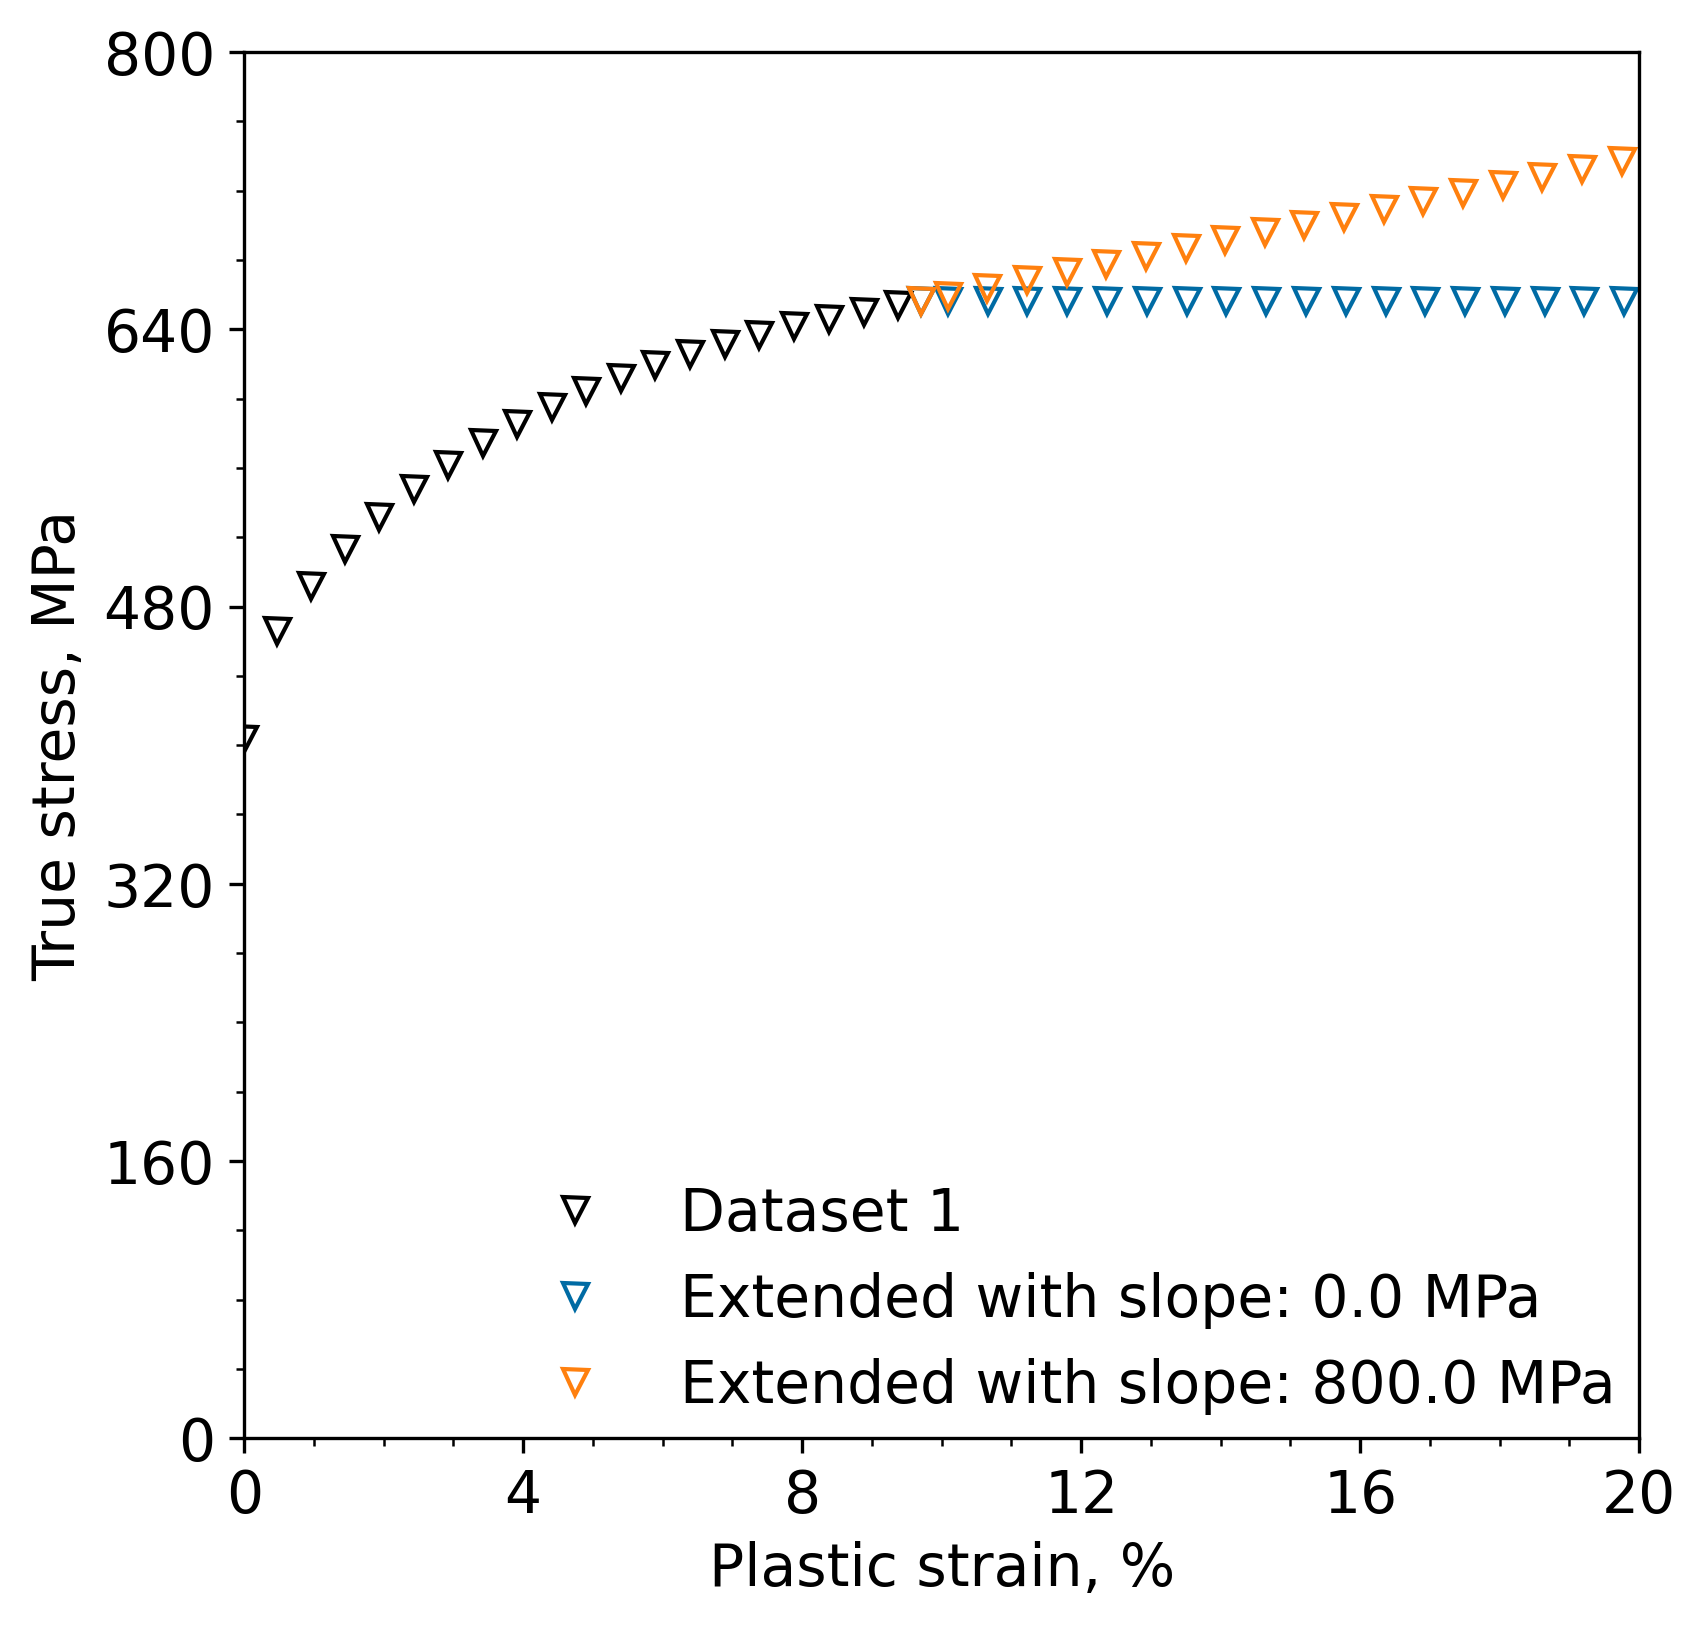
\includegraphics[width=\linewidth, height=0.4\textheight, keepaspectratio]{ABAQUS_SLOPE_COMPARISON}
		\caption{True stress - plastic strain relationship for dataset 1. Test data are shown using black markers. Two parameter values (minimum and maximum) are distingushed using coloured markers.}
		\label{fig:extending_uts}
	\end{figure}

	%%%%%%%%%%%%%%%%%%%%%%%%%%%
	\section{FE Modelling of Tensile Tests}
	\label{h:fem}

	Finite element modelling was conducted using Abaqus 2021~\cite{DASSAULT2021}.
	Analyses were conducted using Abaqus/Explicit, a dynamics based solution, with a mass scaling factor of 10 to reduce computation time.
	The model was meshed using axisymmetric elements.
	A total of 4664 elements were used.
	Each element in the gauge section represents approximately 0.09~mm.

	The experimental tensile test geometry was represented as shown in Figure~\ref{fig:fe_model}.
	The use of a 2D geometry reduces the computational expensive associated with the simulation.
	To predispose the FE model to neck in the central gauge length a small imperfection was introduced to the bottom right hand corner as shown in Figure~\ref{fig:fe_model}.

	\begin{figure}[!htbp]
		\centering
		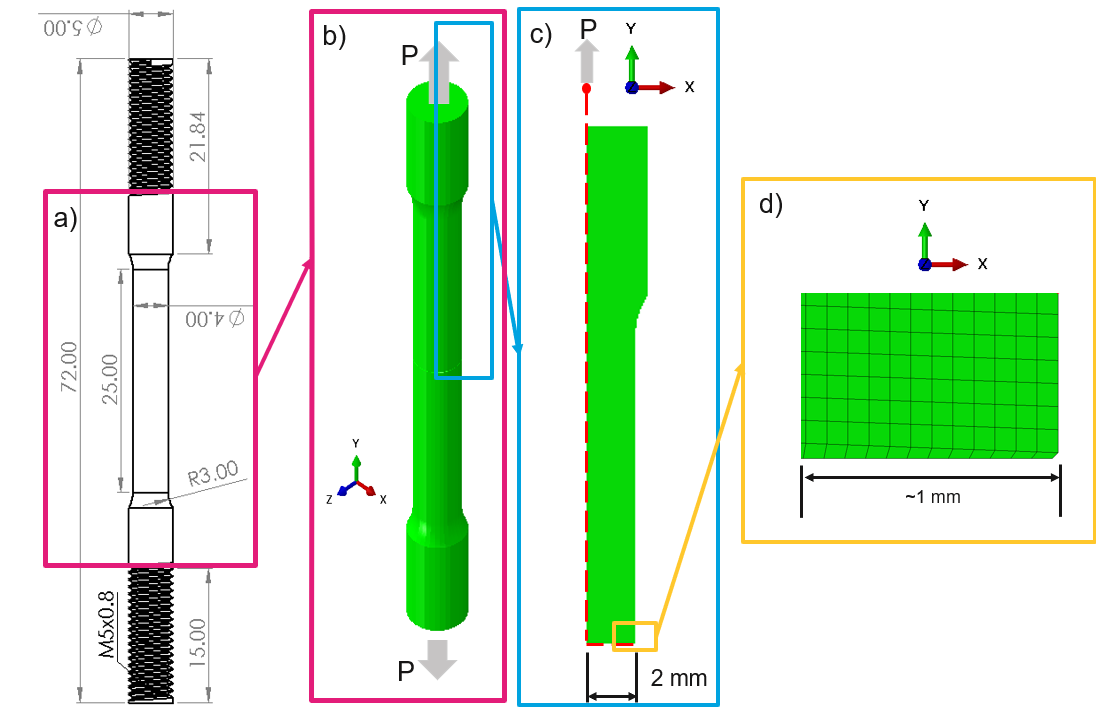
\includegraphics[width=\linewidth, height=0.5\textheight, keepaspectratio]{MODEL_3D_2D}
		\caption{Illustration demonstrating the axisymmetric FE model. A small imperfection, shown in the yellow highlighted region, was modelled to ensure failure occurred in the midsection of the gauge length.}
		\label{fig:fe_model}
	\end{figure}

	Boundary conditions were applied along the symmetry planes (shown by the red dashed lines in Figure~\ref{fig:fe_model}).
	A reference node (red point shown in Figure~\ref{fig:fe_model}) was coupled to the surface of the geometry and loading was applied through displacement control.

	Within the FE simulation linear material behaviour was defined using the $E$ and Poisson's Ratio ($\nu=0.3$).
	Non-linear material behaviour was provided as an array of plastic strain versus true-stress ($^*$PLASTIC in Abaqus).
	To model material degradation due to ductile damage the GTN model was applied (see Section~\ref{h:damage_model}).

	Displacement data was taken from the reference node shown in Figure~\ref{fig:fe_model}.
	The applied load was calculated by summing the vertical reaction force in elements located along the X symmetry plane.

	%%%%%%%%%%%%%%%%%%%%%%%%%%%
	\section{Results and Discussion}
	\label{h:results}
 	As discussed, three data sets have been analysed.
	The minimum MAPE selected is 2\% and the procedure described in Figure~\ref{fig:bo_flowchart} is applied until this MAPE is reached.
	Abaqus simulations are preformed in sequence with 4 CPUs.
	Typically, this framework requires at least 150 finite element simulations with the full parameter selection taking approximately 4 hours.
	The framework was executed on a laptop with 4 Intel i7 CPUs and 32 gigabytes of RAM.
	Not all CPUs are required for the framework, other applications (e.g.\ Microsoft office) are sufficiently supported while the framework runs in the background.
	The lowest MAPE, $1.56~$\%, was found for dataset 1.

	The comparison between data and simulation is shown in Figure~\ref{fig:bo_result} for the three datasets.
 	Figure~\ref{fig:dataset1} shows that the simulated output is in good agreement with experimental data over the full displacement range although simulated forces are slightly underestimated compared with the experiment in the range $1.3 \leq \Delta u \leq 2.2$~mm.
	Similarly Dataset 2 (Figure~\ref{fig:dataset2}) shows good agreement between simulated and experimental data.
	For $\Delta u \geq 2.5$~mm simulated results for Dataset 2 slightly overestimate the force compared to the experiment.
	The overestimation is most notable at the final displacement point.

	%%% compare BO implicit data to experiment
	\begin{figure}[!htbp]
		\begin{minipage}[b]{0.5\linewidth}
			\centering
			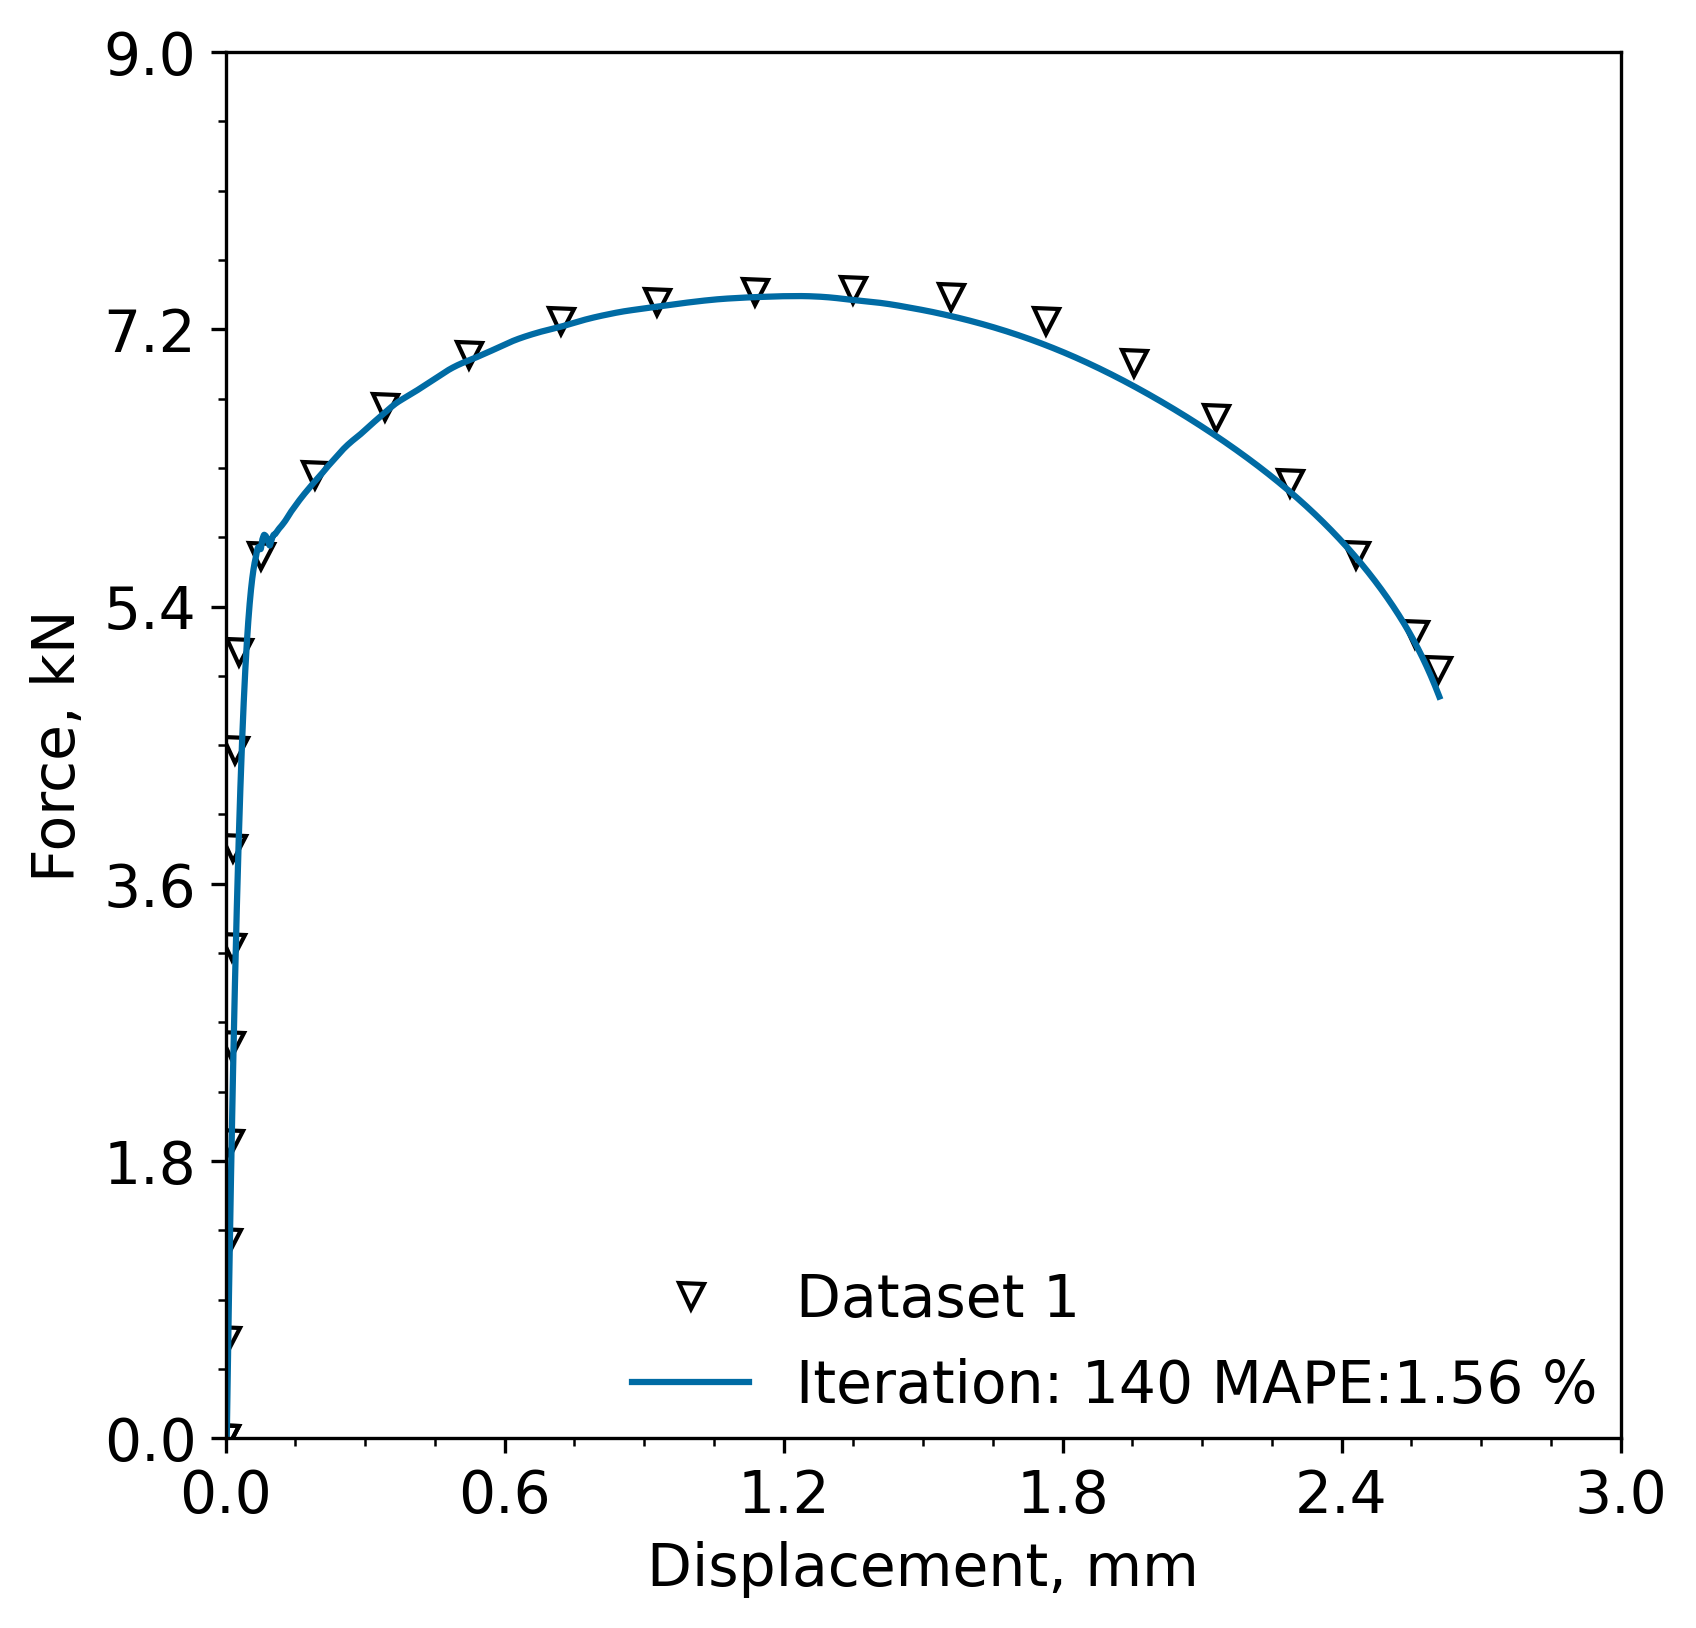
\includegraphics[width=\textwidth, height=0.45\textheight, keepaspectratio]{P91_20_2_FASTEST_ITERATION}
			\subcaption{Dataset 1}
			\label{fig:dataset1}
		\end{minipage}
	\hspace{0.2cm}
		\begin{minipage}[b]{0.5\linewidth}
			\centering
			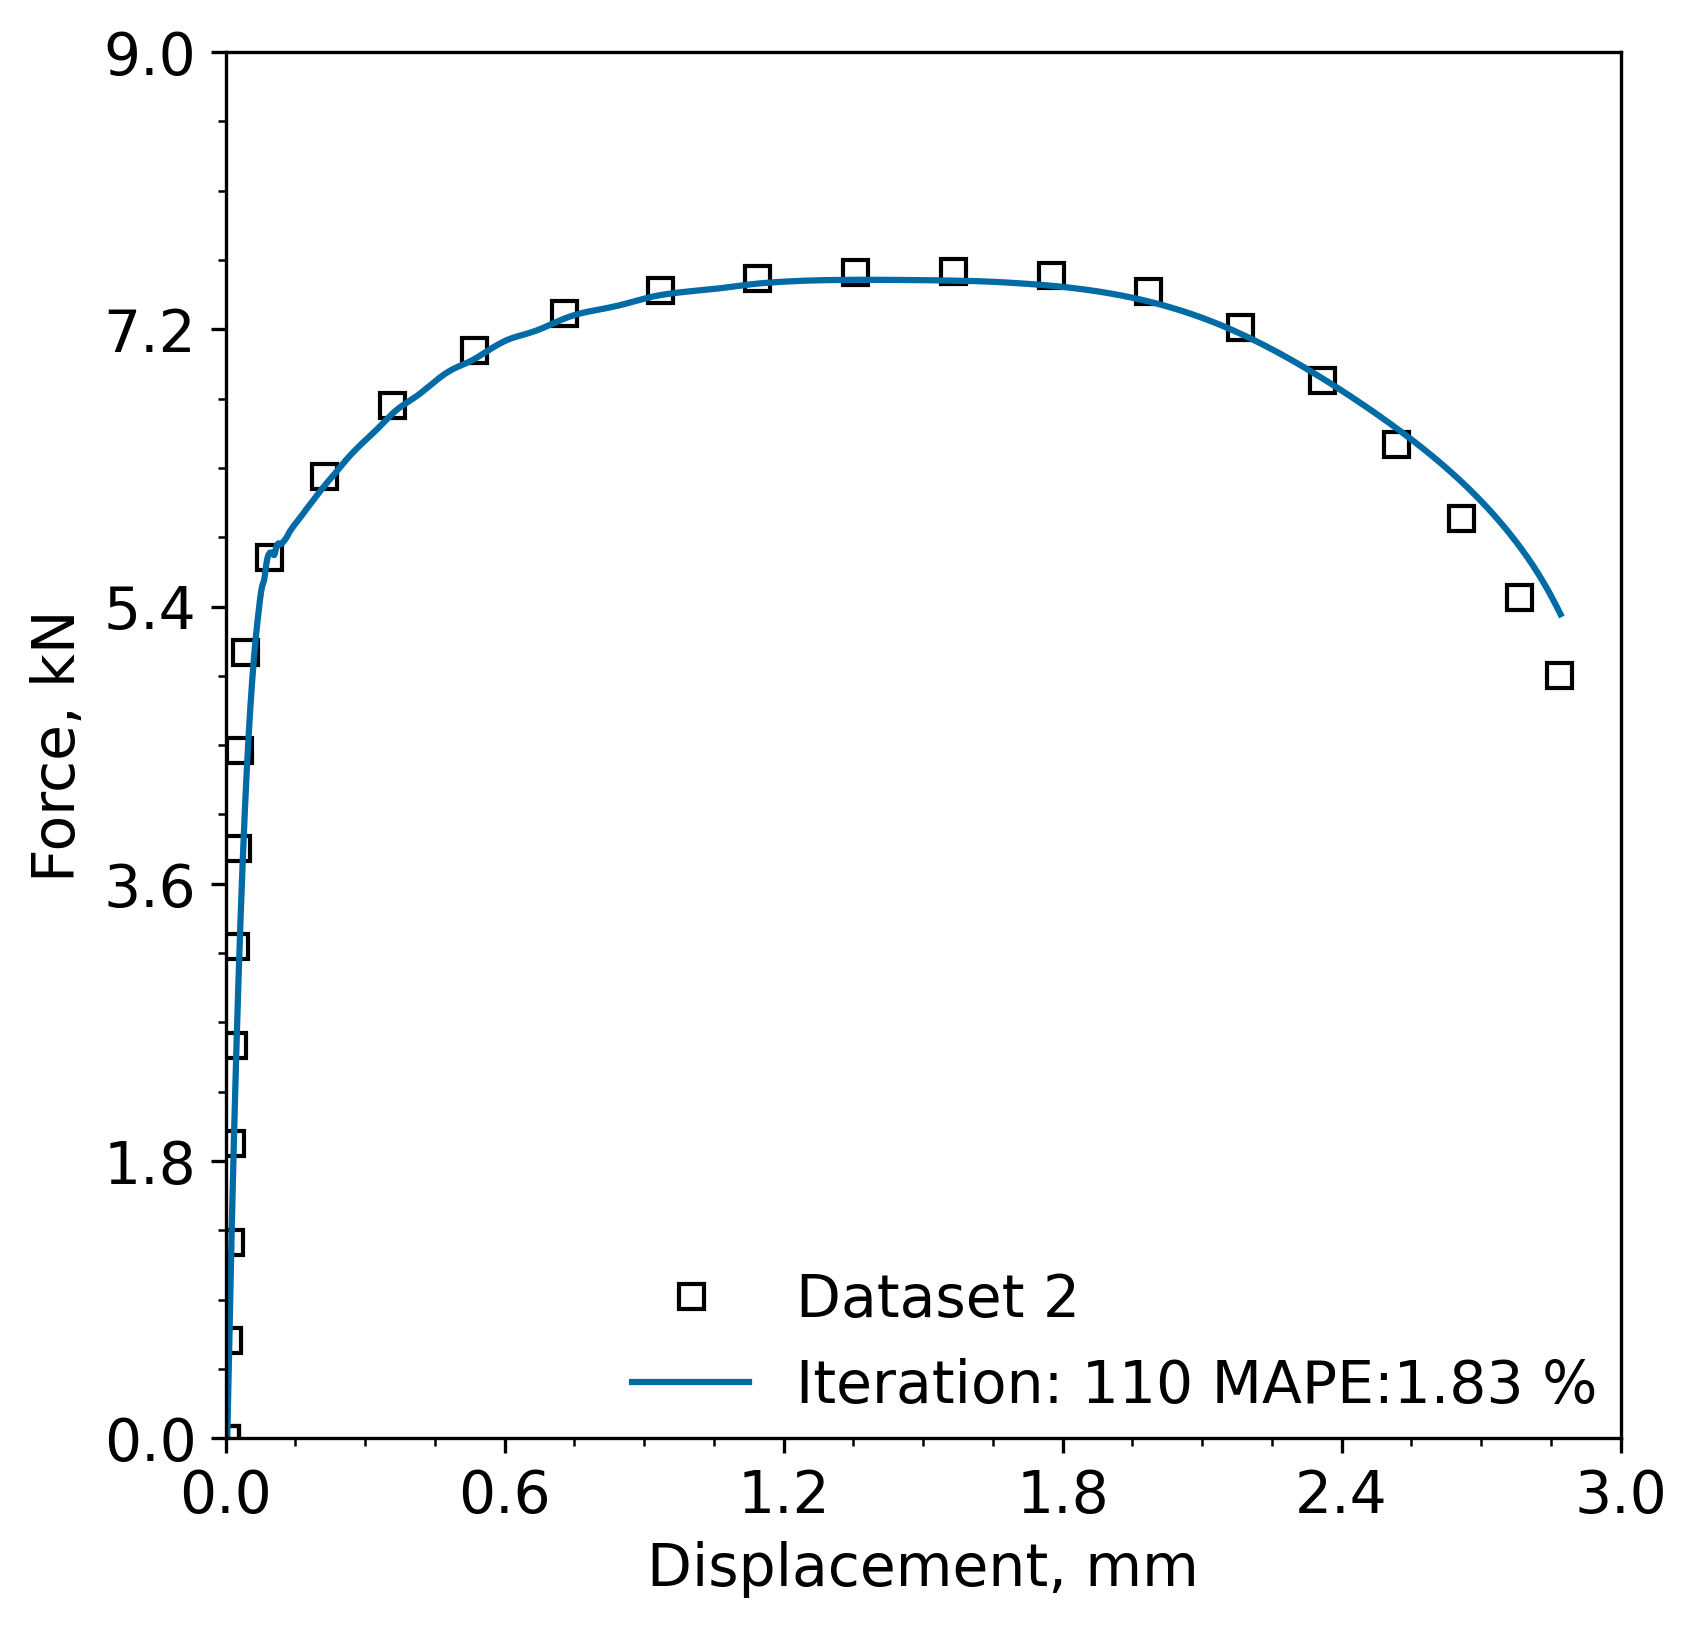
\includegraphics[width=\textwidth, height=0.45\textheight, keepaspectratio]{P91_20_1_FASTEST_ITERATION}
			\subcaption{Dataset 2}
			\label{fig:dataset2}
		\end{minipage}%%
	\vspace{0.2cm}
		\begin{minipage}[b]{\linewidth}
			\centering
			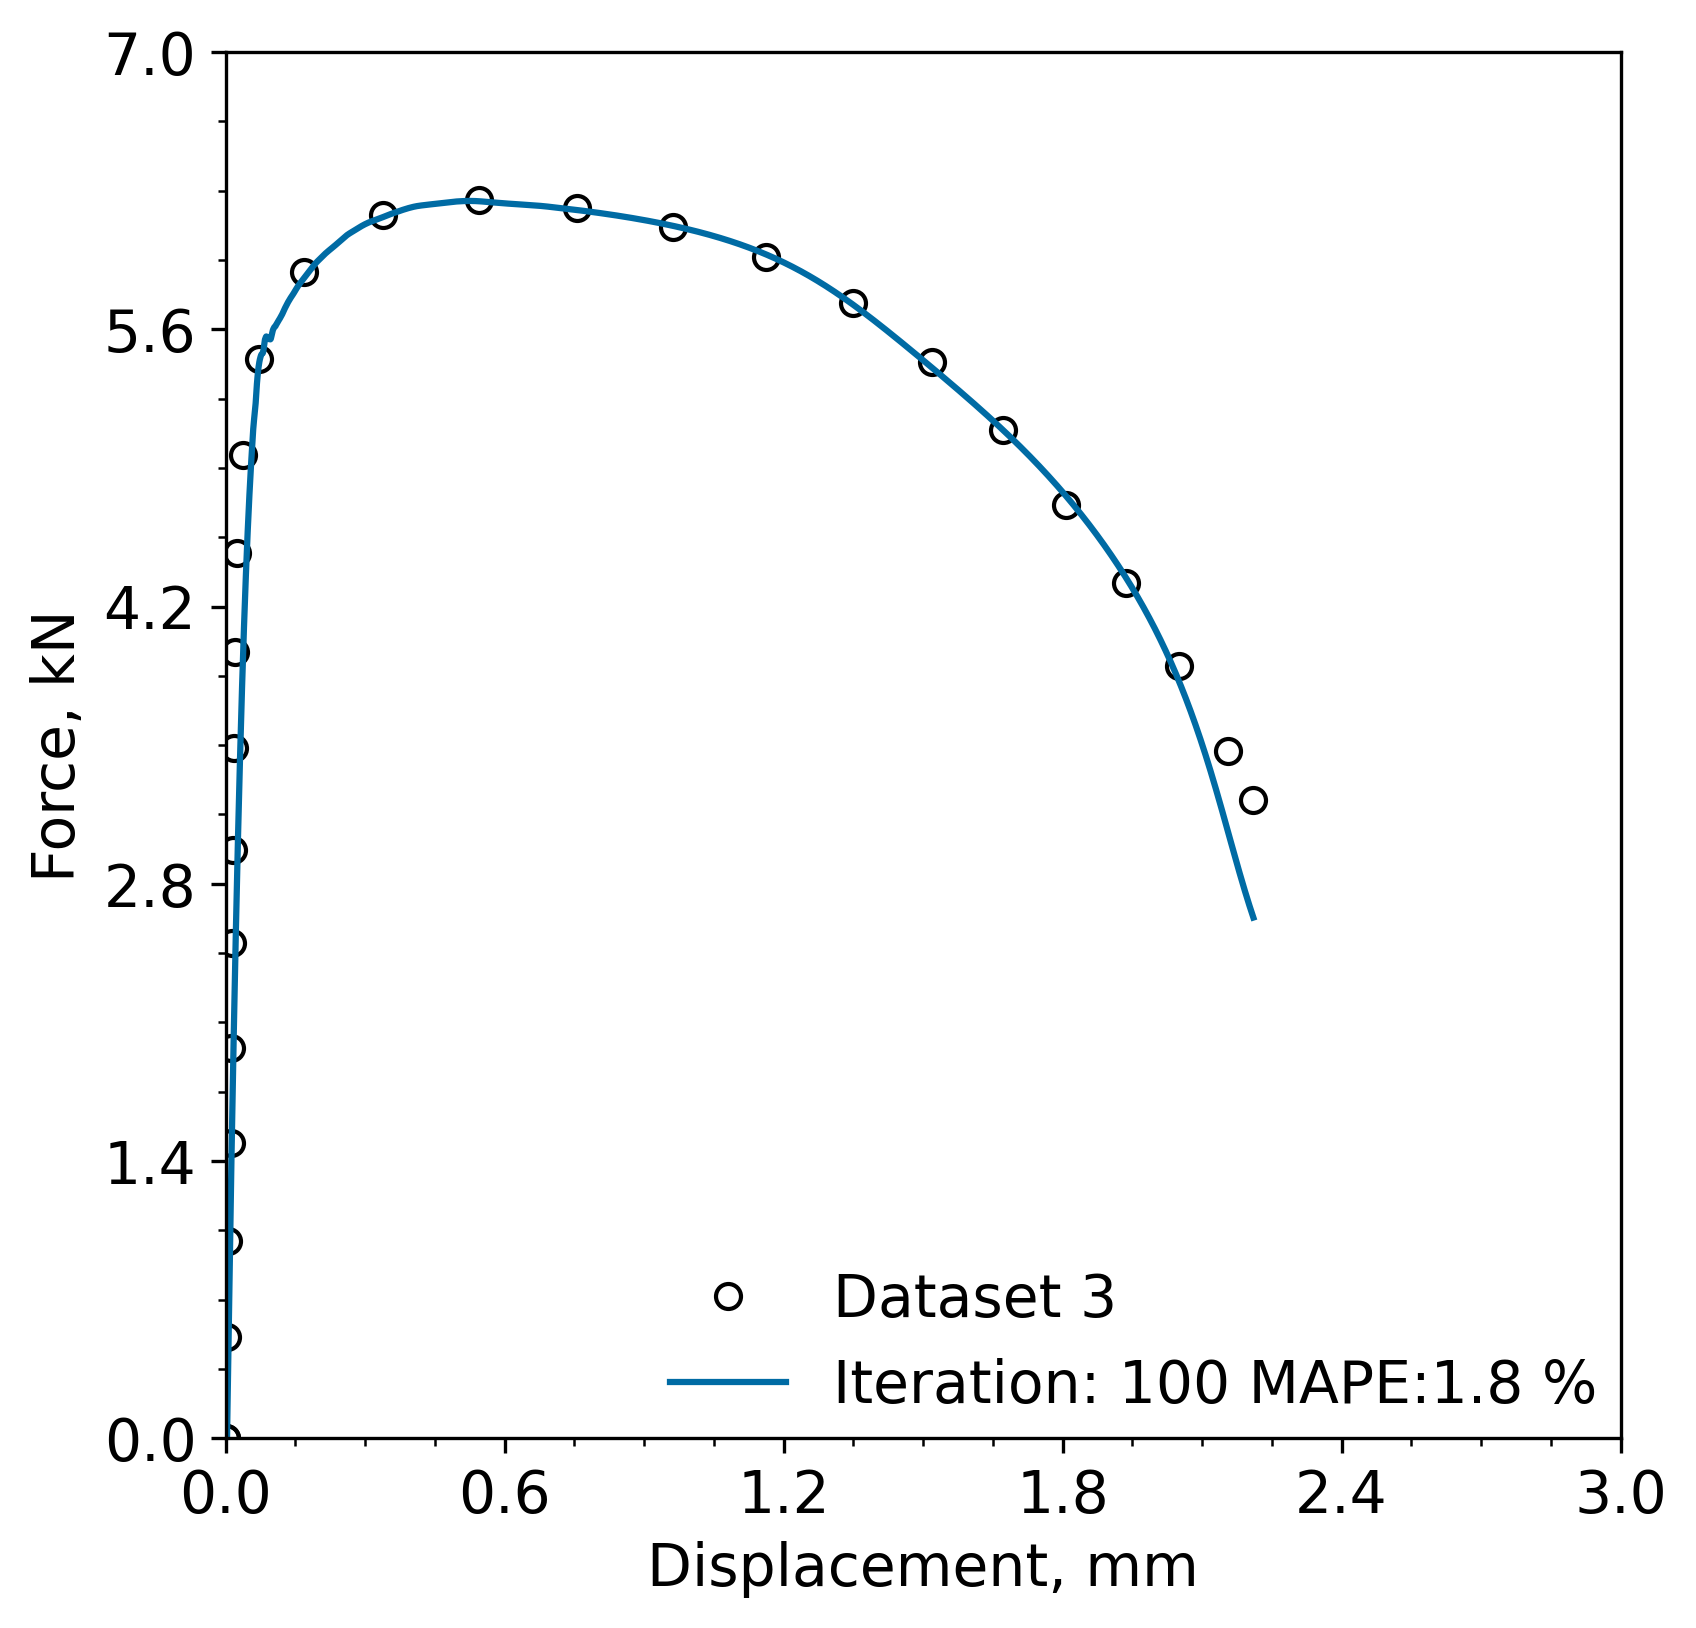
\includegraphics[width=0.5\textwidth, height=0.45\textheight, keepaspectratio]{P91_500_FASTEST_ITERATION}
			\subcaption{Dataset 3}
			\label{fig:dataset3}
		\end{minipage}~\caption{Comparison of experimental test data to simulated output for Dataset 1~(\ref{fig:dataset1}), Dataset 2~(\ref{fig:dataset2}), and Dataset 3~(\ref{fig:dataset3}). Parameter values are shown in Table~\ref{tab:bo_parameter_values}.}
	\label{fig:bo_result}
	\end{figure}
	The parameter values selected by the BO framework are provided in Table~\ref{tab:bo_parameter_values} for each of the three datasets analysed.

	\begin{table}[!htbp]
\centering
\caption{Bayesian optimisation framework parameter values for each of the three datasets analysed. }
\label{tab:bo_parameter_values}
\begin{tabular}{lccc}
\toprule
\textbf{Parameter} & \textbf{Dataset 1} & \textbf{Dataset 2} & \textbf{Dataset 3} \\
\midrule
$N_O$ & \multicolumn{3}{c}{500}\\
$N_R$ & \multicolumn{3}{c}{50,000}\\
%\multirow{2}{*}{\parbox{1.8cm}{Optimisation samples}} & \multicolumn{3}{c}{500}\\
%\\
%\multirow{2}{*}{\parbox{1.8cm}{Random samples}} & \multicolumn{3}{c}{50,000}\\
%\\
\midrule
%\textbf{$q_1$} &    1.3324 &    1.1684 &    1.1820 \\
%\textbf{$q_2$} &    0.9952 &    0.9667 &    0.9699 \\
%\textbf{$q_3$} &    2.2949 &    1.4071 &    2.0007 \\
%\textbf{$\epsilon_N$} &    0.2900 &    0.3467 &    0.3720 \\
%\textbf{$s_N$} &    0.1671 &    0.1856 &    0.1214 \\
%\textbf{$f_N$} &    0.0387 &    0.0848 &    0.0471 \\
%\textbf{$f_0$} &    1.374 \times 10^{-3} &    1.344 \times 10^{-3} &    1.310 \times 10^{ -3} \\
%\textbf{$m$} &  534.13 &  725.39 &  421.41 \\
%{MAPE} &    1.56 &    1.83 &    1.80 \\
%{Iteration number} &  140 &  110 &  100 \\
%% 4 SIGNIF FIGURES
\textbf{$q_1$} &    1.332 &    1.168 &    1.182 \\
\textbf{$q_2$} &    9.952\times10^{-1} &    9.667\times10^{-1} &    9.699\times10^{-1} \\
\textbf{$q_3$} &    2.295 &    1.407 &    2.001 \\
\textbf{$\epsilon_N$} &    2.900\times10^{-1} &    3.467\times10^{-1} &    3.720\times10^{-1} \\
\textbf{$s_N$} &    1.671\times10^{-1} &    1.856\times10^{-1} &    1.214\times10^{-1} \\
\textbf{$f_N$} &    3.869\times10^{-2} &    8.481\times10^{-2} &    4.706\times10^{-2} \\
\textbf{$f_0$} &    1.370 \times 10^{-3} &    1.340 \times 10^{-3} &    1.310 \times 10^{ -3} \\
\textbf{$m$} &  534.1 &  725.4 &  421.4 \\
{MAPE} &    1.563 &    1.827 &    1.799 \\
{$N_j$} &  140 &  110 &  100 \\
\bottomrule
\end{tabular}
\end{table}


	The datasets analysed are for the same batch of material.
	The tests for dataset 1 and 2 have been carried out under identical conditions, while the test for dataset 3 has been carried out at a different temperature.
	The statistical nature of materials testing, often termed material scatter, has been widely acknowledged in the field of material science~\cite{OCONNOR2022}.
	Given the difficultly in experimentally deriving material values and considering the statistical nature of material performance, it may be that machine learning methods such as the ones employed here are more appropriate for defining such parameters.
	It is interesting to note that parameter $m$, the slope of the extrapolated true stress-true strain curve was found to differ significantly between datasets 1 and 2.
	The optimised parameter $m$ for datasets 1 was found to be 534~MPa while that for dataset 2 was found to be 725~MPa.
	Both datasets were tested under identical conditions and, as shown in Figure~\ref{fig:exp_test_results}, are broadly similar up to a displacement of $\approx 1.3$~mm after which they begin to diverge.

	It is also interesting to note that for all three datasets the parameter $f_0$, representing the initial void volume fraction of the material are very similar.
	Generally the initial void volume fraction is assumed to be applicable to all test samples taken from a single batch of material which is consistent with what is observed here.
	However, comparing parameters $\varepsilon_N$, $S_N$ and $f_N$ across the three datasets presented in Table~\ref{tab:bo_parameter_values}, there are significant differences.
	These parameters control how many voids nucleate under a given loading condition and, as such, are expected to be material specific rather than specimen specific.

	In terms of the fitting parameters ($q_1$, $q_2$ and $q_3$) it is common practise among the engineering community to fix $q_3 = q_1^2$~\cite{ABBASI2011,ROUSSELIER2019, YAN2021} this is based on assumptions made in the original model ~\cite{TVERGAARD1981a}.
	In this work $q_3$ was not constrained as a function of $q_1$.
	Interestingly, despite the freedom of the BO framework to select any value of $q_3$, Table~\ref{tab:bo_parameter_values} shows that dataset 2 found a value of $q_3=1.4071$ which is analogous to $q_1^2=1.3652$.
	Other fitting parameters ($q_1$ and $q_2$) are broadly similar when comparing across datasets.
	Given the complex nature of the material model and the close relationship between some parameters it is difficult to state with any certainty what impact any individual parameter has had on simulated output.

	\subsection{Effect of varying BO hyperparameters}
	\label{h:unique}

	To assess the effect of hyperparameter selection on the model parameters multiple analyses on dataset 1 were preformed.
	For each analysis the number of random and/or optimisation samples ($N_R$ and $N_0$, respectively) were reduced as shown in Table~\ref{tab:hyper_parameter_values}.
	Reducing $N_R$ reduces the precision of the input parameters which increases model uncertainty.
	The $N_O$ defines how many evaluations of the acquisition function are conducted, this controls the level of uncertainty specifically related to the acquisition function.
	Results are plotted in Figure~\ref{fig:unique}.
	\begin{figure}[!htbp]
		\centering
		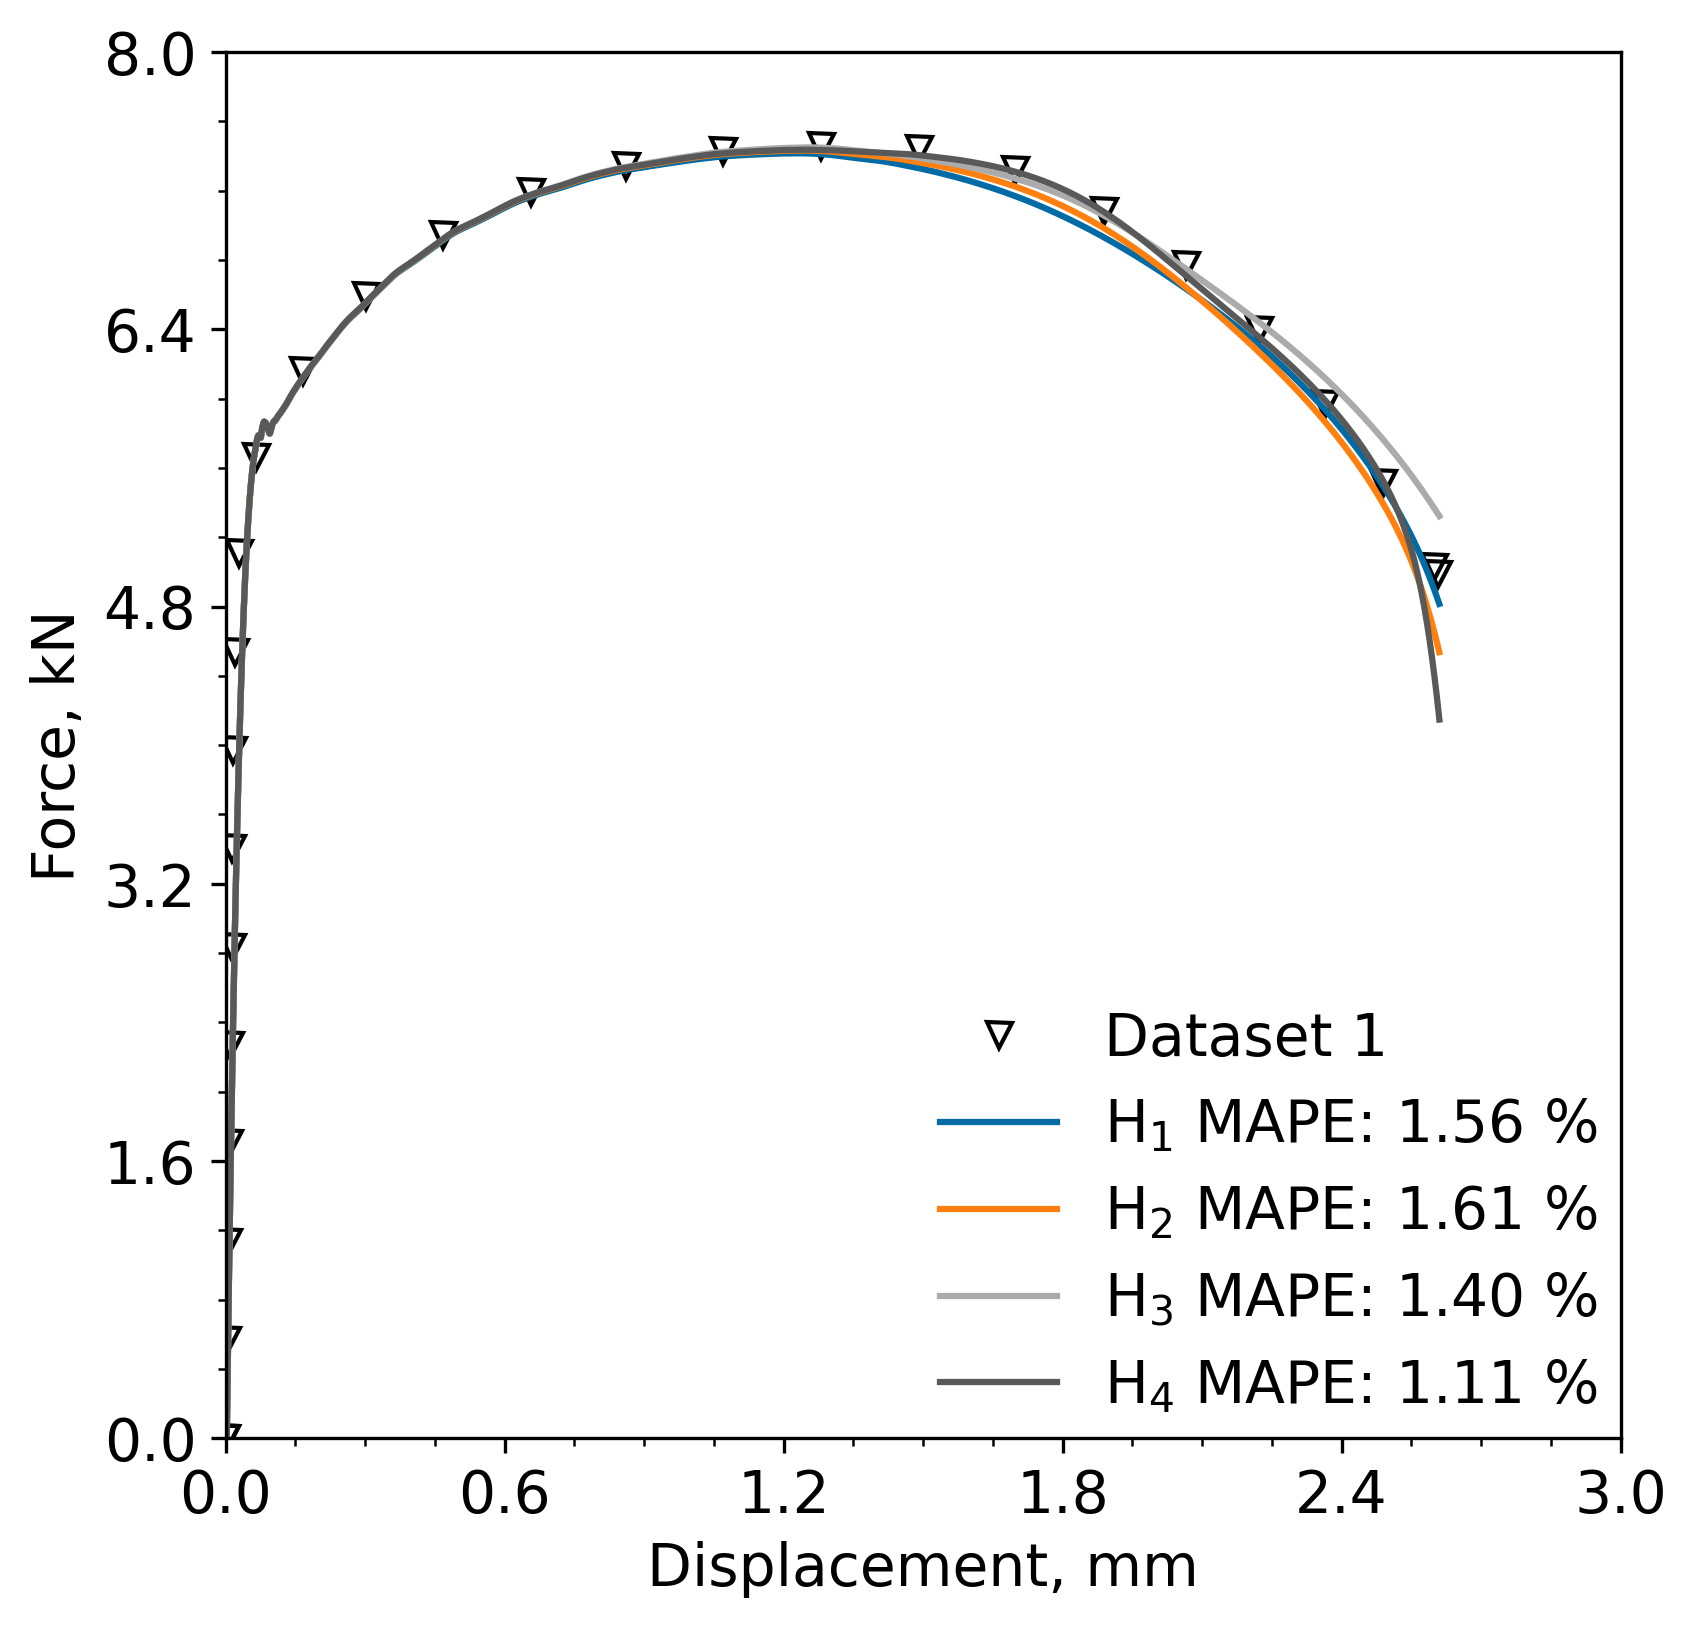
\includegraphics[width=\linewidth, height=0.4\textheight, keepaspectratio]{HYPERPARAMETERS}
		\caption{Plot of force versus displacement showing experimental data and simulated output for various hyperparameters.}
		\label{fig:unique}
	\end{figure}

	\begin{table}[!htbp]
\centering
\caption{Bayesian optimisation framework parameter values for dataset 1. The effect of hyperparameter settings on GTN parameter values. }
\label{tab:hyper_parameter_values}
\begin{tabular}{lcccc}
\toprule
\textbf{Parameter} & \textbf{$H_1$} & \textbf{$H_2$} & \textbf{$H_3$} & \textbf{$H_4$}\\
\midrule
$N_O$ & 500 & 100 & 500 & 100\\
$N_R$ & 50,000 & 50,000 & 10,000 & 10,000\\
%\multirow{2}{*}{\parbox{1.8cm}{Optimisation samples}} & \multirow{2}{*}{500} & \multirow{2}{*}{100} & \multirow{2}{*}{500} & \multirow{2}{*}{100}\\
%\\
%\multirow{2}{*}{\parbox{1.8cm}{Random samples}} & \multirow{2}{*}{50,000} & \multirow{2}{*}{50,000} & \multirow{2}{*}{10,000} & \multirow{2}{*}{10,000}\\
%\\
\midrule
%\textbf{$q_1$} & 1.3324 & 1.1775 & 1.2910 & 1.1578 \\
%\textbf{$q_2$} & 0.9952 & 1.0214 & 0.9547 & 1.0365 \\
%\textbf{$q_3$} & 2.2949 & 1.3443 & 2.2535 & 1.0702 \\
%\textbf{$\epsilon_N$} & 0.2900 & 0.3598 & 0.3517 & 0.3331 \\
%\textbf{$s_N$} & 0.1671 & 0.1580 & 0.1001 & 0.1234 \\
%\textbf{$f_N$} & 0.0387 & 0.0577 & 0.0309 & 0.0759 \\
%\textbf{$f_0$} & 1.374\times10^{-3} & 1.431\times10^{-3} & 1.412\times10^{-3} & 1.308\times10^{-3} \\
%\textbf{$m$}   & 534.13 & 542.79 & 514.54 & 621.85 \\
%{MAPE}         & 1.56 & 1.61 & 1.40 & 1.11 \\
%{Iteration number} & 140 & 133 & 46 & 130 \\
%% SIGNIFICANT FIGURES 4
\textbf{$q_1$} & 1.332 & 1.178 & 1.291 & 1.158 \\
%\textbf{$q_2$} & 0.9952 & 1.021 & 0.9547 & 1.037 \\
\textbf{$q_2$} & 9.952\times10^{-1} & 1.021 & 9.547\times10^{-1} & 1.037 \\
\textbf{$q_3$} & 2.295 & 1.344 & 2.254 & 1.070 \\
\textbf{$\epsilon_N$} & 2.900\times10^{-2} & 3.598\times10^{-1} & 3.519\times10^{-1} & 3.331\times10^{-1} \\
\textbf{$s_N$} & 1.671\times10^{-1} & 1.580\times10^{-1} & 1.001\times10^{-1} & 1.234\times10^{-1} \\
\textbf{$f_N$} & 3.869\times10^{-2} & 5.769\times10^{-2} & 3.086\times10^{-2} & 7.594\times10^{-2} \\
\textbf{$f_0$} & 1.370\times10^{-3} & 1.431\times10^{-3} & 1.412\times10^{-3} & 1.309\times10^{-3} \\
\textbf{$m$}   & 534.1 & 542.8 & 514.5 & 621.9 \\
{MAPE}         & 1.563 & 1.614 & 1.398 & 1.105 \\
{$N_j$} & 140 & 133 & 46 & 130 \\
\bottomrule
\end{tabular}
\end{table}



	Figure~\ref{fig:unique} shows that excellent agreement with experimental data is achieved for the four different hyperparameter choices but, it may be noted from Table~\ref{tab:hyper_parameter_values} that the model parameters can depend significantly on hyperparameter selection.
	Given that excellent agreement was achieved for all four analyses this implies that the problem does not have a unique solution.
	That is to say that multiple combinations of the eight model parameters potentially provide good agreement to experimental data.

	The lowest MAPE, $1.11$\% was found for analysis $H_4$ where $N_R$and $N_O$ were 10,000 and 100, respectively.
	Comparing the model parameters ($q_1$, $q_2$ etc.) for the four analyses shows that $H_4$ deivates considerably from $H_1$.
	$H_1$, as it has the highest $N_R$ and $N_O$, is considered the most precise of the analyses investigated here.
	Comparing parameter $m$ in analyses $H_1$ (534.13~MPa) and $H_4$ (621.85~MPa) shows a difference of almost 100~MPa.
	In terms of the expected change, and considering the parameter range, the deviation across analyses is significant.
	It is therefore not unexpected that the remaining parameter values, those specific to the GTN model, also differ.
	This outcome supports the non-uniqueness of the problem.

	Comparing $H_1$ and $H_2$ in Table~\ref{tab:hyper_parameter_values} indicates how reducing $N_O$ affects the analysis.
	While individual model parameters change slightly, overall both analyses provide similar measures of MAPE and result in load-displacement traces similar to the experimental data (Figure~\ref{fig:unique}).
	It should be noted that $H_2$ resulted in a slightly higher MAPE, 1.61\%, compared to that of $H_1$, 1.56\%.
	The higher measure of MAPE for $H_2$ is as expected given that the reduced $N_O$ effectively reduces the amount of statistical information known about the black box function resulting in less accuracy.

	Comparing $H_1$ and $H_3$ in Table~\ref{tab:hyper_parameter_values} enables the effect of reducing $N_R$ to be assessed.
	Here it is shown that fitting parameters $q_1$, $q_2$ and $q_3$ are broadly similar.
	Other parameters, specifically nucleation related terms $s_N$ and $f_N$, exhibit differences with $H_3$ having smaller values compared to $H_1$.
	The effect of the reduction in these parameters is also notable in Figure~\ref{fig:unique} where comparing $H_1$ and $H_3$ shows that $H_3$ deviates from $H_1$ at $2.0 \leq \Delta \leq 2.7$~mm.
	In essence the lower nucleation parameters seen in analysis $H_3$ reduced the nucleation of new voids thus giving a lower rate of damage compared to $H_1$.
	On the whole comparing $H_1$ and $H_3$ indicates that reducing $N_R$ did not significantly affect the model output.
	In fact comparing $H_1$ and $H_2$ to $H_3$ shows that lower $N_R$ provided a more accurate result (i.e.\ lower MAPE) in a significantly shorter timescale (iteration number 46).
	While this may appear initially surprising it simply means that lower values of $N_R$ did not overtly effect the mean calculation of the block-box function.
	Analysis $H_4$ shows output associated with a reduction in both the $N_O$ and $N_R$.
	Interestingly $H_4$ has the lowest MAPE, 1.11\%, however the number of iterations (130) is similar to those required for the $H_1$ and $H_2$ analyses.

	It is difficult to state with any certainty which, if any, of the analyses in Table~\ref{tab:hyper_parameter_values} would be considered the most `appropriate'.
	The issue of non-uniqueness in GTN model parameter values has been highlighted by others~\cite{KIRAN2014, CHAHBOUB2019}.
	One method of limiting the GTN parameters is to introduce other, cracked, specimen geometries such as single edge notch bend (SENB) or compact tension (CT) geometries.
	Cracked geometries are subject to considerable local stress triaxiality that inhibits plastic flow and promotes void growth~\cite{BROCKS1995}.
	As the GTN model, Equation~\ref{eq:gtn_yield}, is not specimen specific the parameters of the model should be equally applicable to a uni-axial tensile geometry or a fracture toughness geometry (e.g.\ SENB or CT geometry).
	Theoretically one could integrate several types of geometry to the framework developed here to limit the number of parameter combinations.
	However, the introduction of a cracked geometry causes several complications.
	Numerical simulations of cracked geometries often require contact interactions and specialist meshing techniques which increases model complexity and computational demand.
	While this is certainly within the ability of modern computing ability the increase in computational demand would inevitably increase the required time for BO to define a solution.
	Testing cracked geometries typically requires additional material, expensive and specialist laboratory equipment and expertise in fracture mechanics.
	Where test data are not available the loss function (MAPE) for the cracked geometry cannot be calculated leaving the BO framework, specifically the acquisition function, struggling to rank data.

	%%%%%%%%%%%%%%%%%%%%%%%%%%%
	\section{Conclusions}
	\label{h:conclusions}

	\begin{itemize}
		\item A Bayesian optimisation framework successfully determined an array of eight material parameter values that, when applied to a ductile damage model simulation, produced an accurate representation of experimental tensile data with a mean average percentage error (MAPE) of less than 2\%.
		\item The framework is fully autonomous requiring minimal user interaction with the combined machine learning-finite element tool typically provides calibration values in less than four hours. This compares favourably with typical time spent on trial-and-error calibration for this model.
		\item The ductile model parameter values are found to be non-unique and it is shown that by changing the hyperparameters of the acquistion function, different combinations of ductile damage parameters are obtained, which provide good agreement wih experimental data.
		\item Future work will consider how the BO framework can be adapted to obtain unique model parameters.
	\end{itemize}

	A preprint of this research is available~\cite{OCONNOR2023}.
	Additional supplementary information such as data files and code are available from zenodo~\url{https://doi.org/10.5281/zenodo.7686217}.


	%%%%%%%%%%%%%%%%%%%%%%%%%%%
	\section{Ackowledgements}
	\label{h:acknowledgements}

	This work was funded by the European Union through the Marie Sk{\l}owodska-Curie Actions grant number 101028291.
	The contributions of William Brennan, a University of Limerick undergraduate student, is thanked for his contributions to earlier versions of the algorithm used in this work.
	We gratefully acknowledge helpful conversations with Dr. Meghana Kshiragar and Gauri Vaidya from the University of Limerick's Lero Centre.
	We also thank the University of Limerick, Mathematics Applications Consortium for Science and Industry (MACSI) group for their insightful and supportive comments surrounding this research.

%% If you have bibdatabase file and want bibtex to generate the
%% bibitems, please use
%
\bibliography{BO_PAPER}
\bibliographystyle{elsarticle-num-names}
	\biboptions{sort&compress}

\end{document}

\endinput
%%
%% End of file `elsarticle-template-num-names.tex